\newpage\subsection*{User Interface Screenshots of the test cases}\label{appendix:testcases}

\newpage

\begin{figure}[htbp]
    \centering
    \begin{subfigure}[b]{0.25\textwidth}
        \centering
        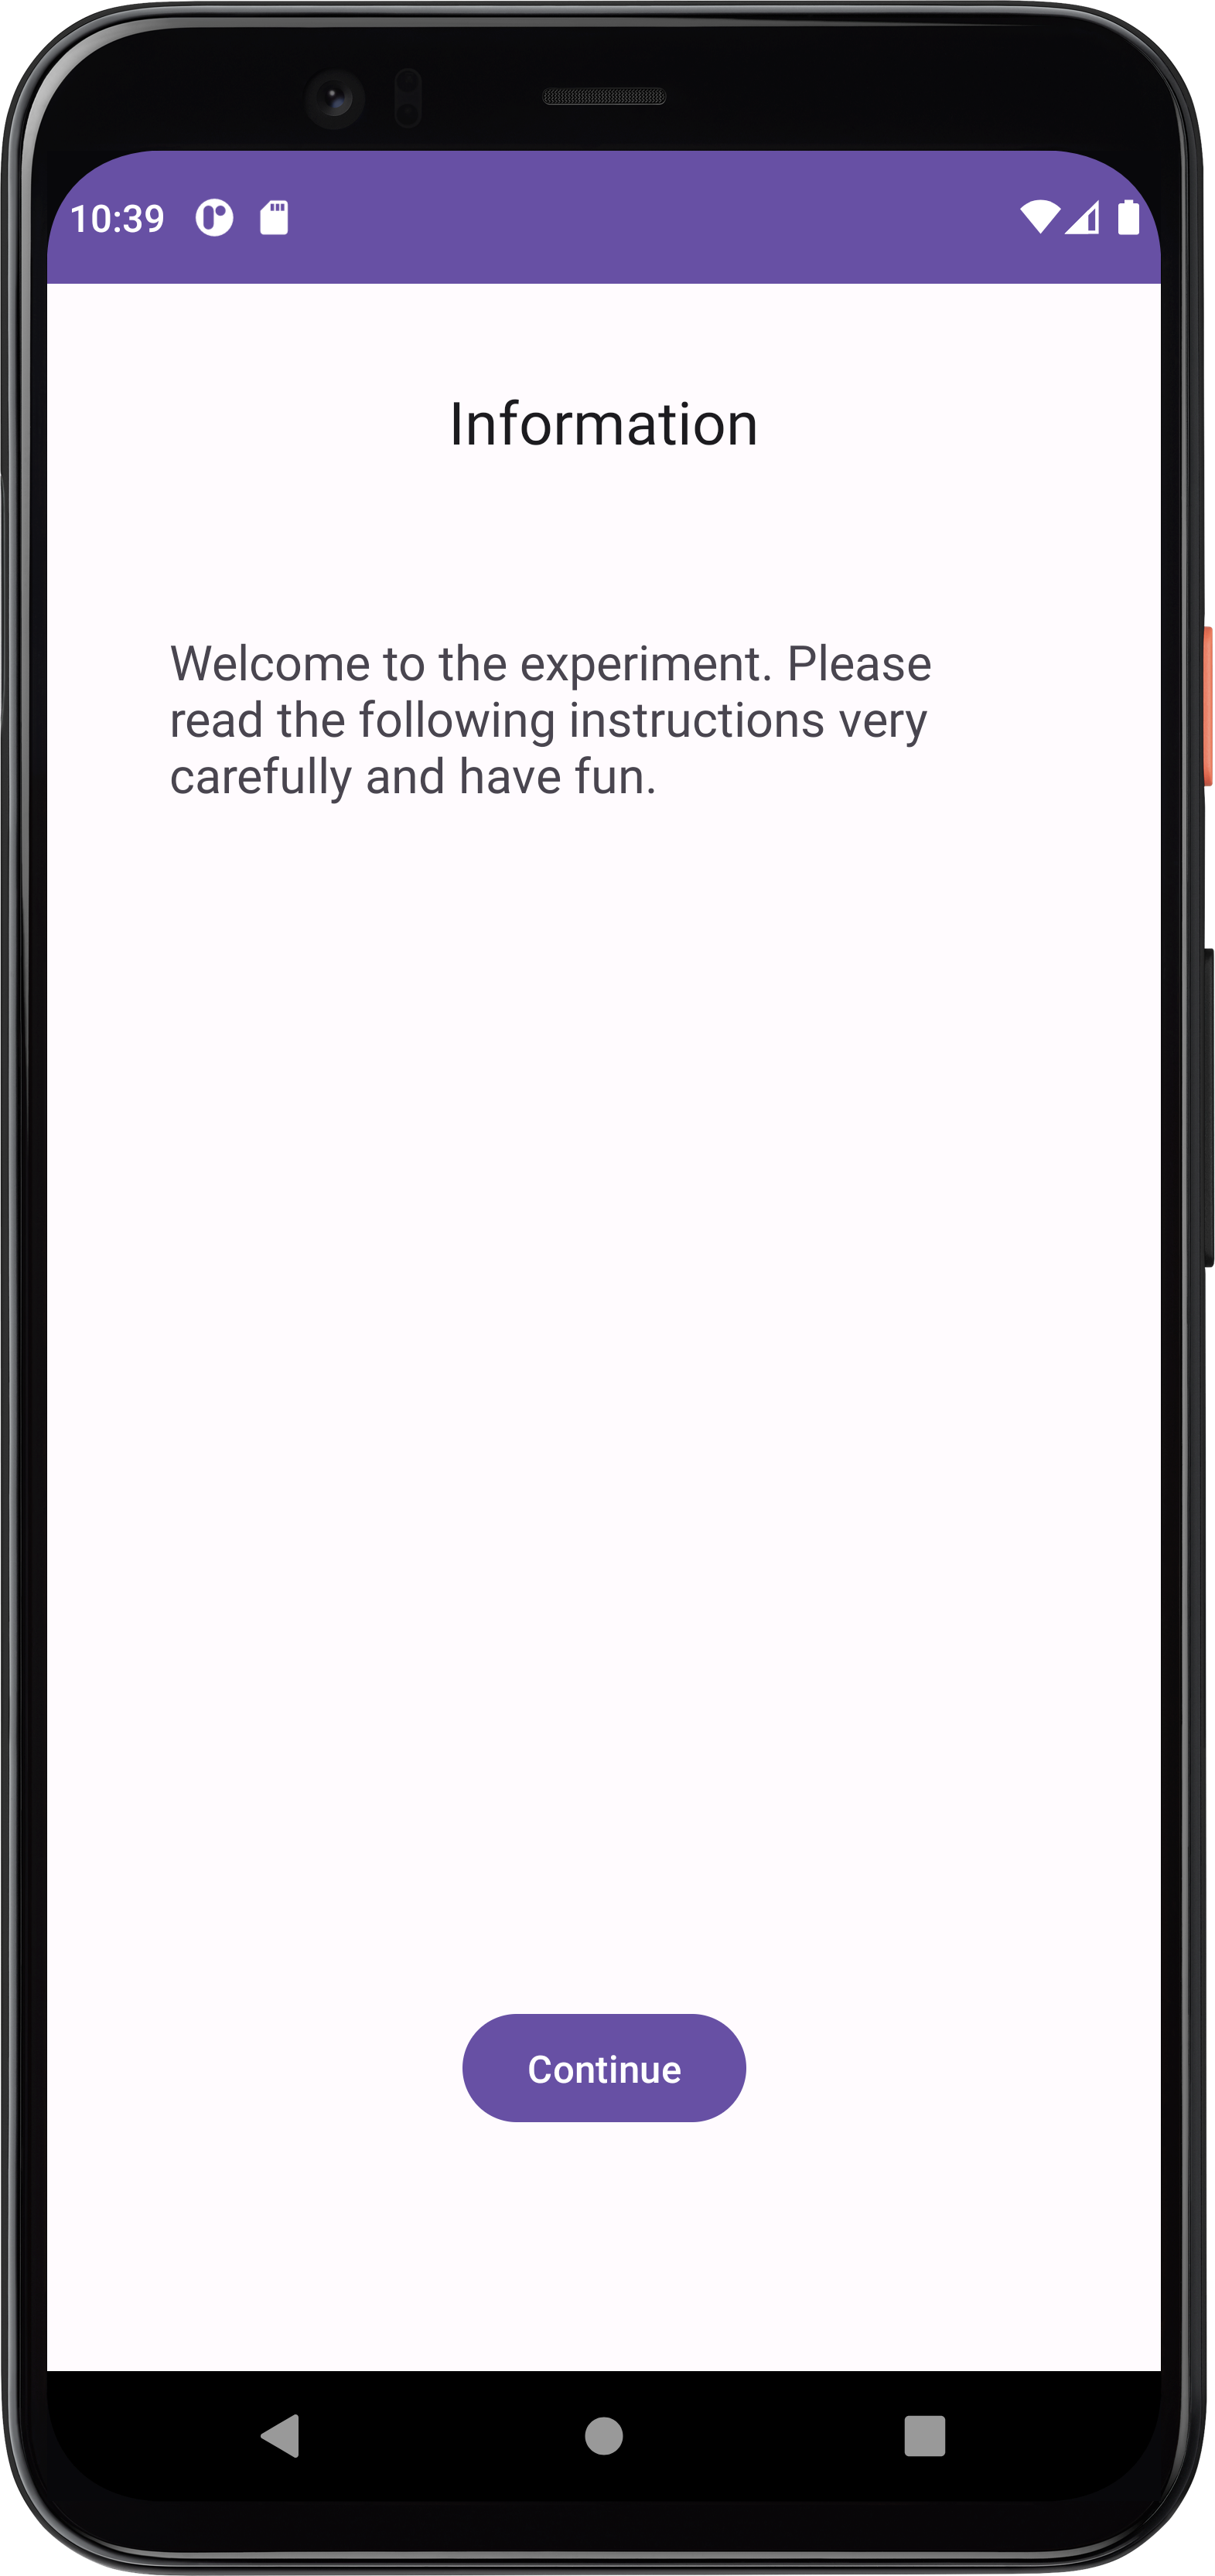
\includegraphics[width=\textwidth]{content/07_evaluation_of_the_solution/Screenshot_StartingScreen.png}
        \caption{Welcome Message}
        \label{subfig:welcomeMessage}
    \end{subfigure}
    \hspace{1cm}
    \begin{subfigure}[b]{0.25\textwidth}
        \centering
        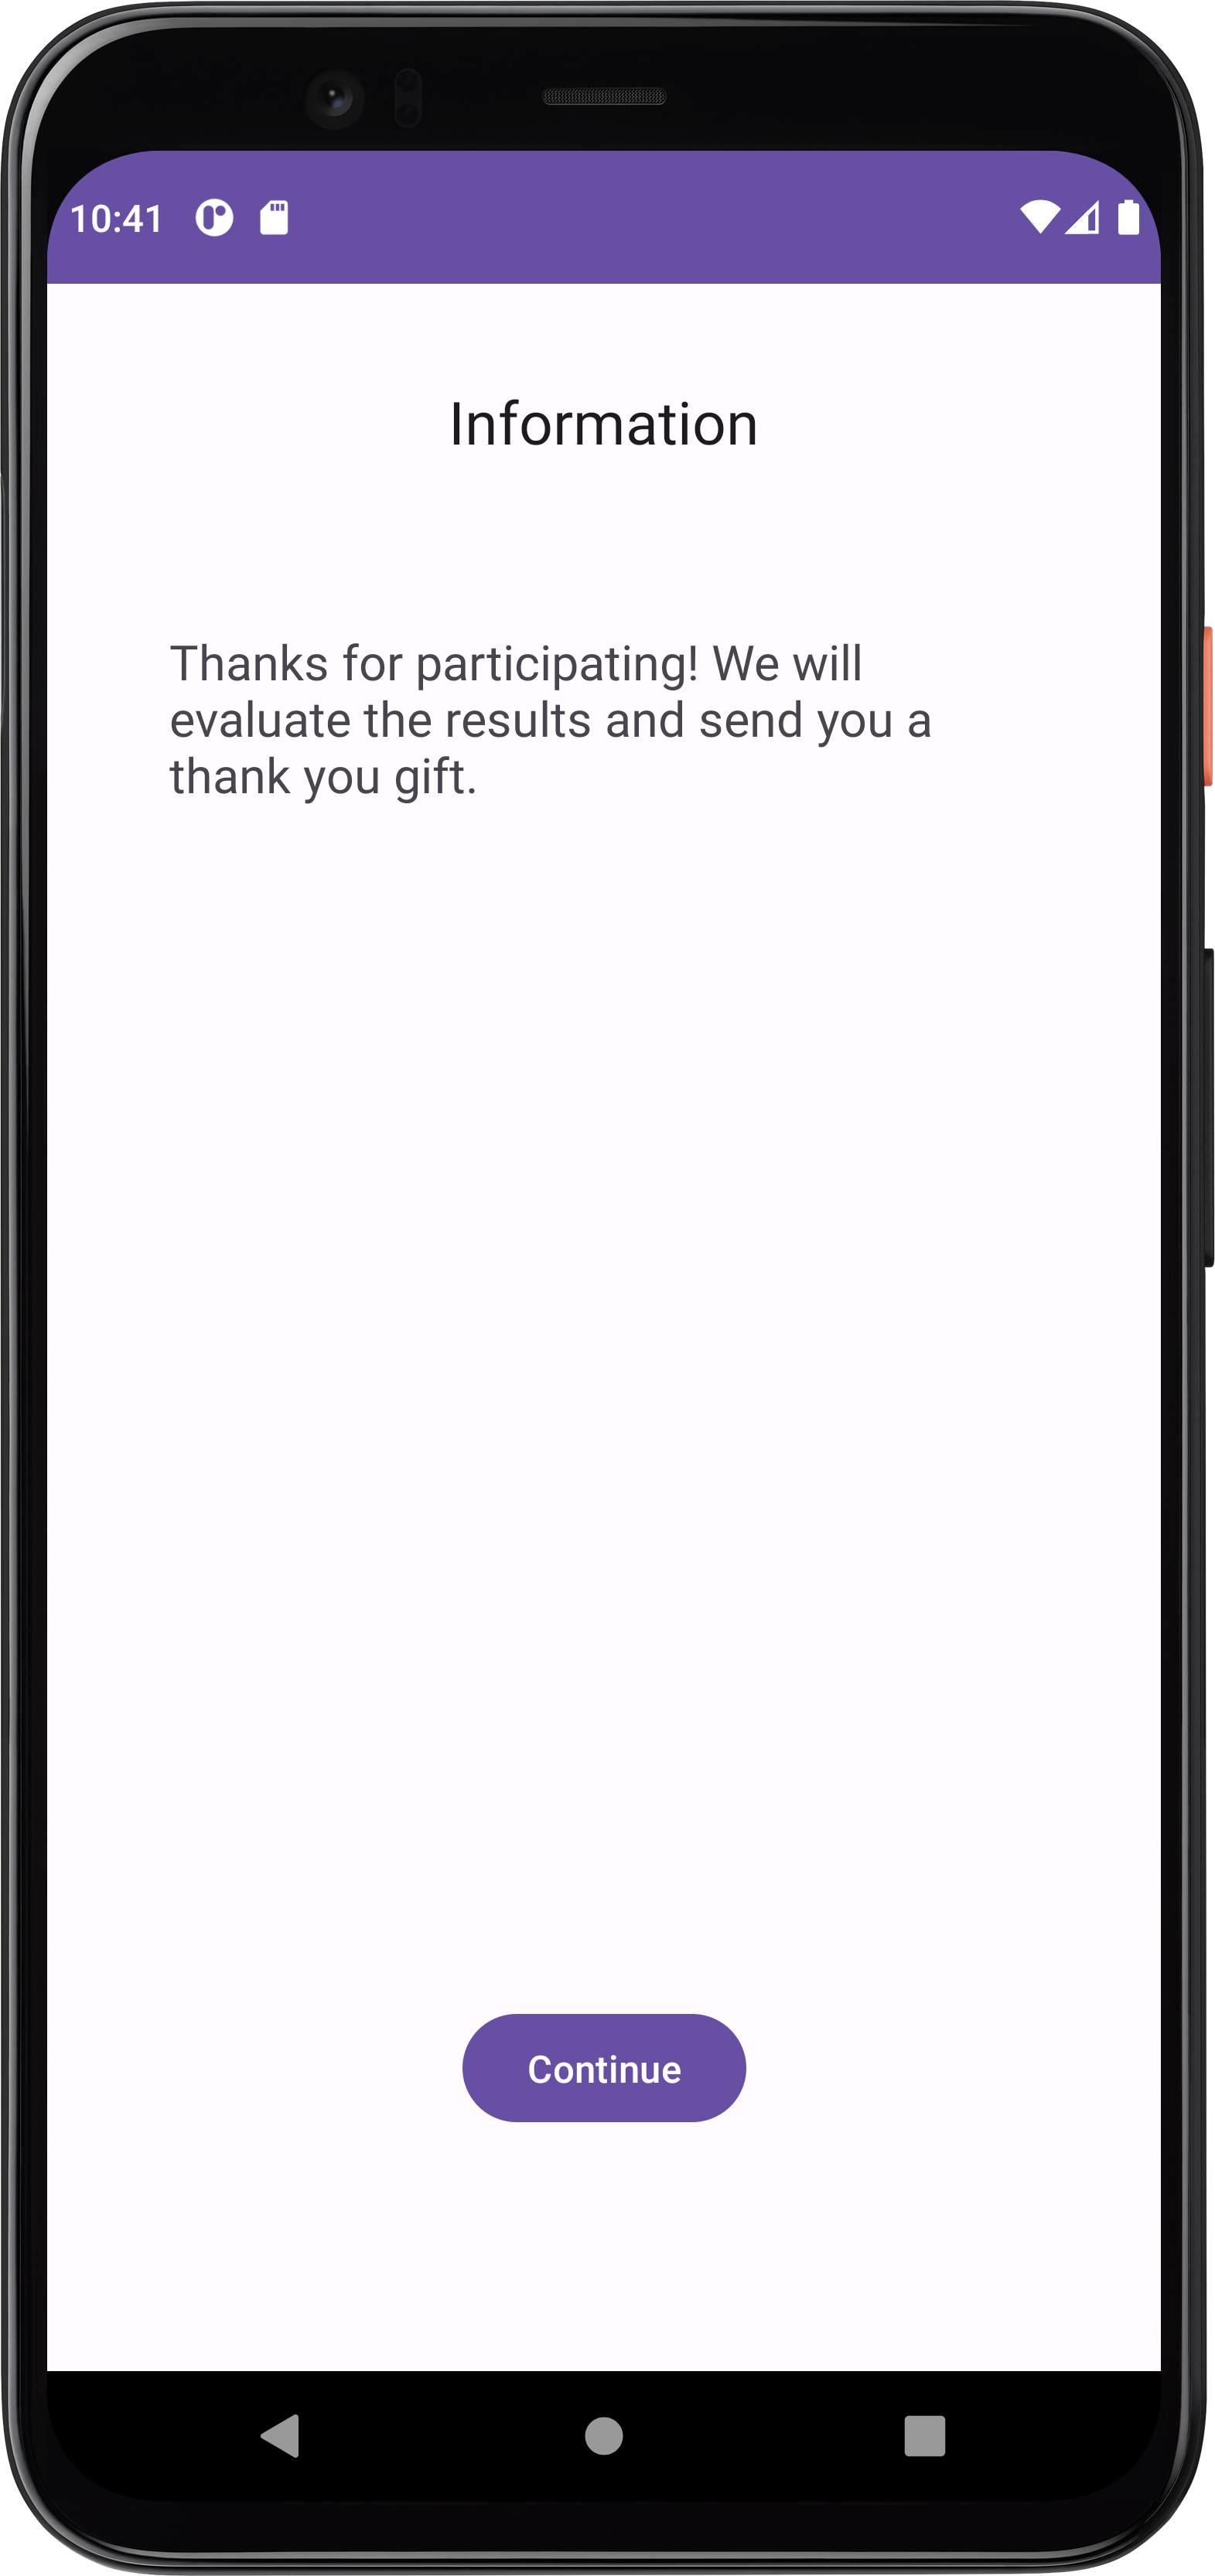
\includegraphics[width=\textwidth]{content/07_evaluation_of_the_solution/Screenshot_GoodbyeMessage.png}
        \caption{Goodbye Message}
        \label{subfig:goodbyeMessage}
    \end{subfigure}
    \caption{User Interface Testcase T1}
    \label{fig:T1}
\end{figure}

\begin{figure}[htbp]
    \centering
    \begin{subfigure}[b]{0.25\textwidth}
        \centering
        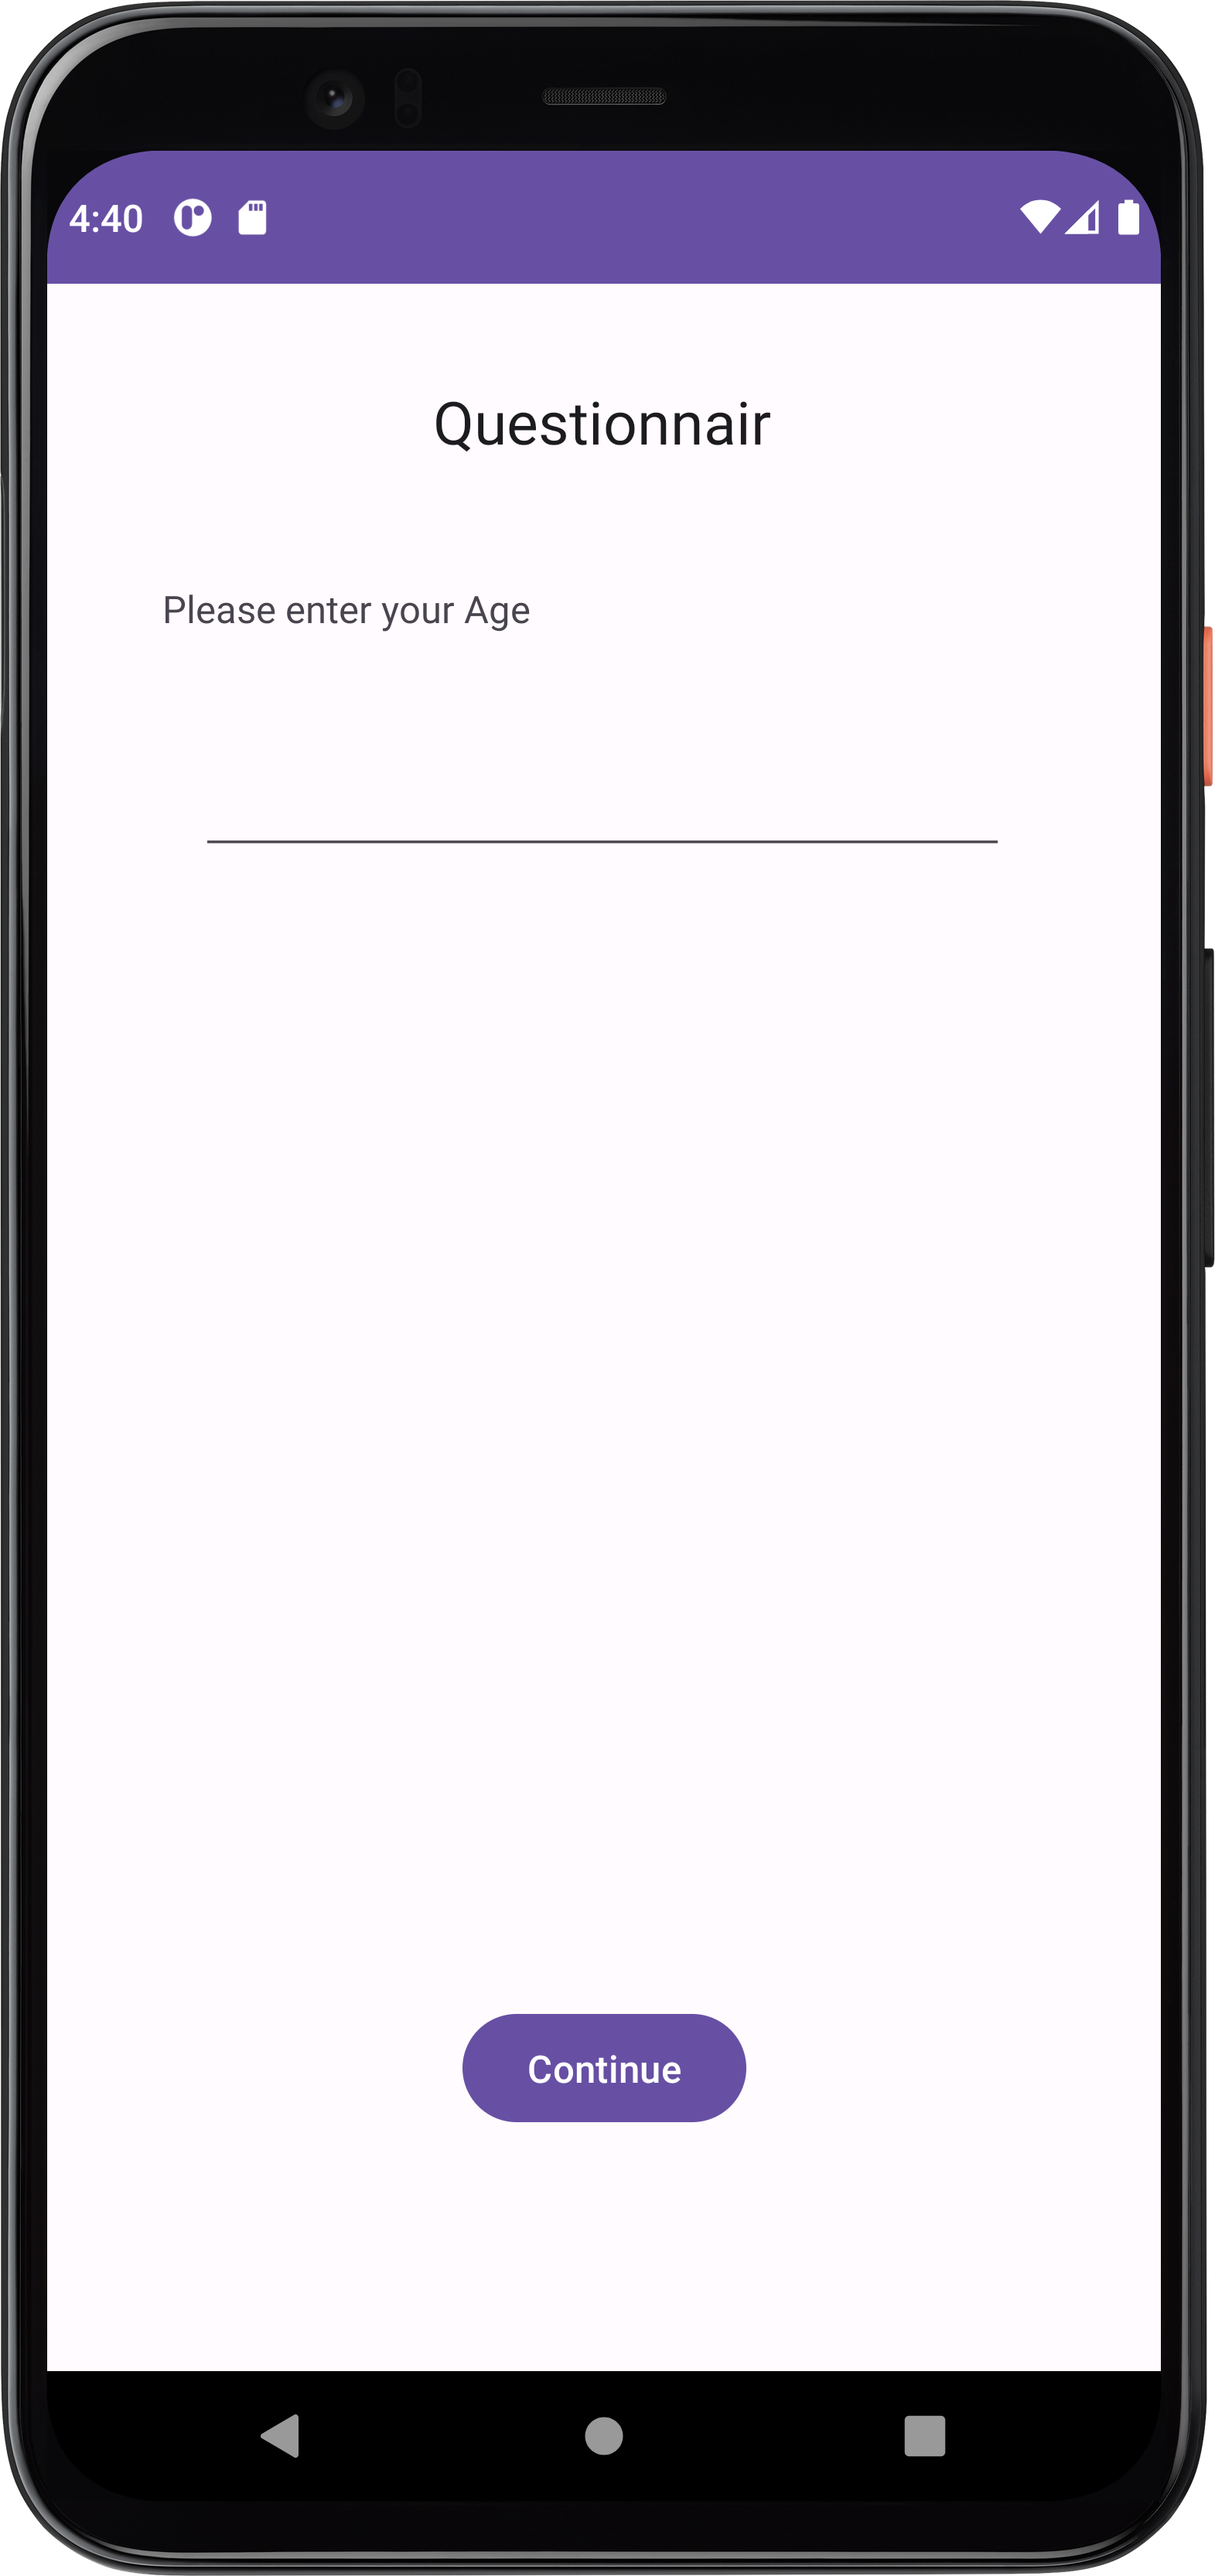
\includegraphics[width=\textwidth]{content/07_evaluation_of_the_solution/Screenshot_T2a.png}
        \caption{Welcome Message}
        \label{subfig:t2a}
    \end{subfigure}
    \hspace{1cm}
    \begin{subfigure}[b]{0.25\textwidth}
        \centering
        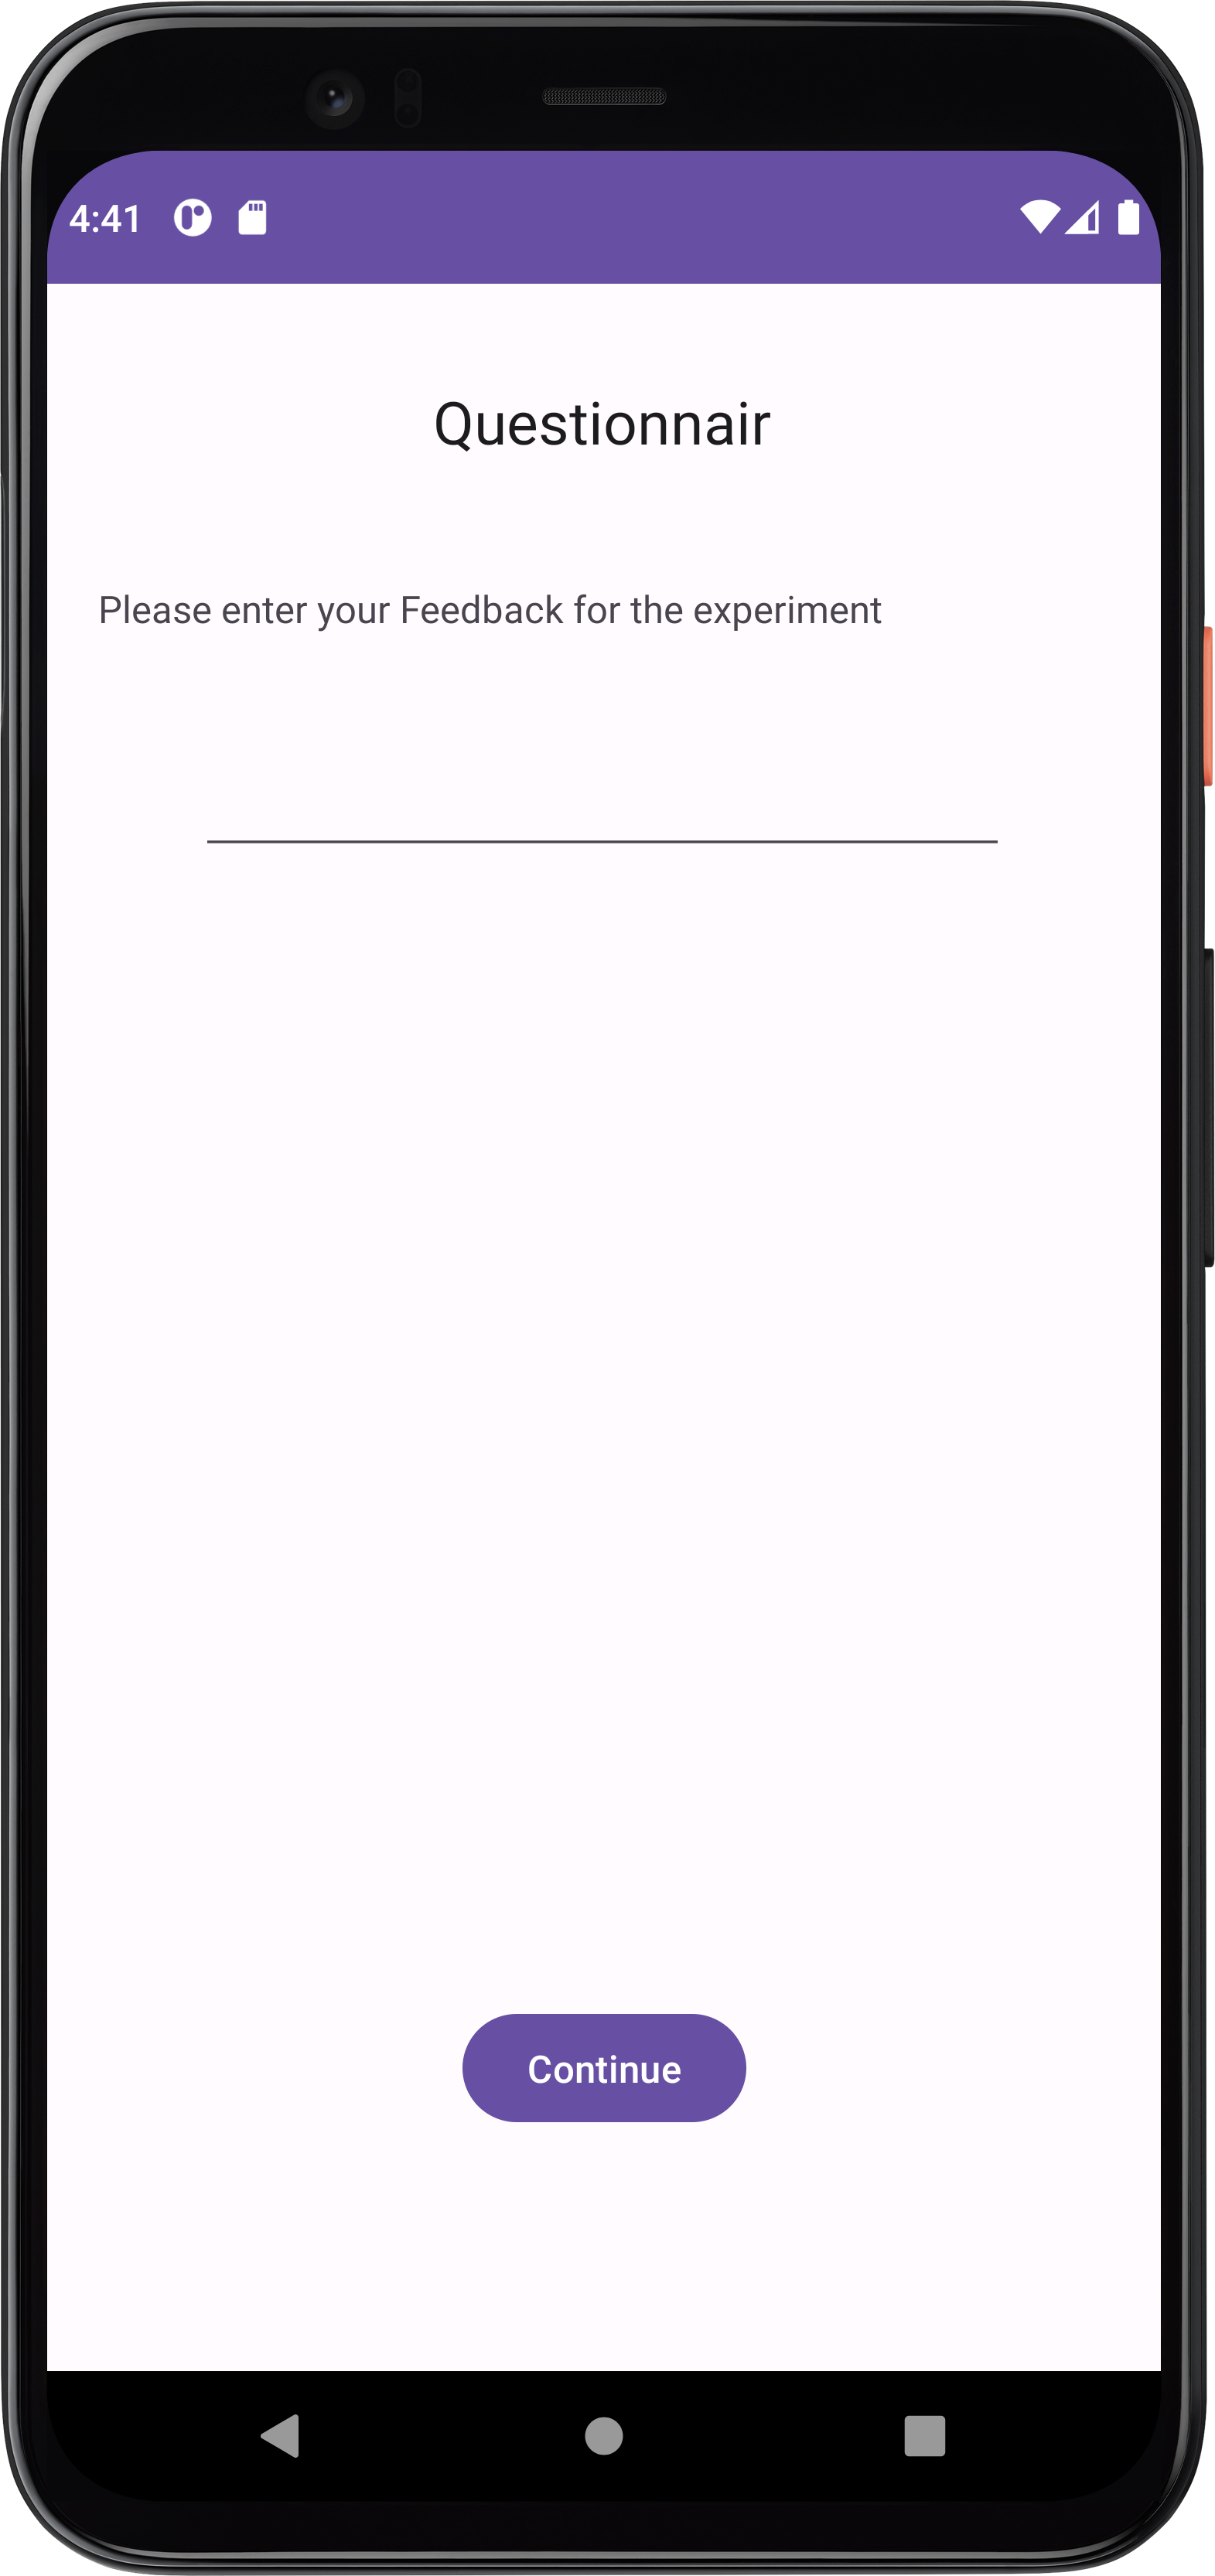
\includegraphics[width=\textwidth]{content/07_evaluation_of_the_solution/Screenshot_T2b.png}
        \caption{Goodbye Message}
        \label{subfig:t2b}
    \end{subfigure}
    \caption{User Interface Testcase T1}
    \label{fig:T2}
\end{figure}


\begin{lstlisting}[language=java,label=t3a,lineskip={0pt}, caption=Collect time needed to conduct experiment (a), basicstyle=\scriptsize, captionpos=b]
    String currentTime = new SimpleDateFormat("HH:mm:ss", Locale.getDefault()).format(new Date());
    LogMetaDataUseCase.getInstance().setMetaData(currentTime);
\end{lstlisting}

\begin{lstlisting}[language=java,label=t3b,lineskip={0pt}, caption=Collect time needed to conduct experiment (b), basicstyle=\scriptsize, captionpos=b]
    long difference = date1.getTime() - date2.getTime();
    LogMetaDataUseCase.getInstance().setMetaData(difference);
\end{lstlisting}

\begin{lstlisting}[language=java,label=t3b,lineskip={0pt}, caption=Collect time needed to conduct experiment (b), basicstyle=\scriptsize, captionpos=b]
    File csvfile = new File(Environment.getExternalStorageDirectory() + "/participantData.csv");
    CSVReader reader = new CSVReader(new FileReader(csvfile.getAbsolutePath()));
    String[] nextLine;
    while ((nextLine = reader.readNext()) != null) {
        // nextLine[] is an array of values from the line
        ParticipantEntity participant = new ParticipantEntity(Integer.parseInt(nextLine[0]));
        participant.setName(nextLine[0]);
        participant.setEducation(nextLine[0]);
        participant.setGender(null);
    
        data.add(participant);
    }
\end{lstlisting}

\begin{figure}[htbp]
    \centering
    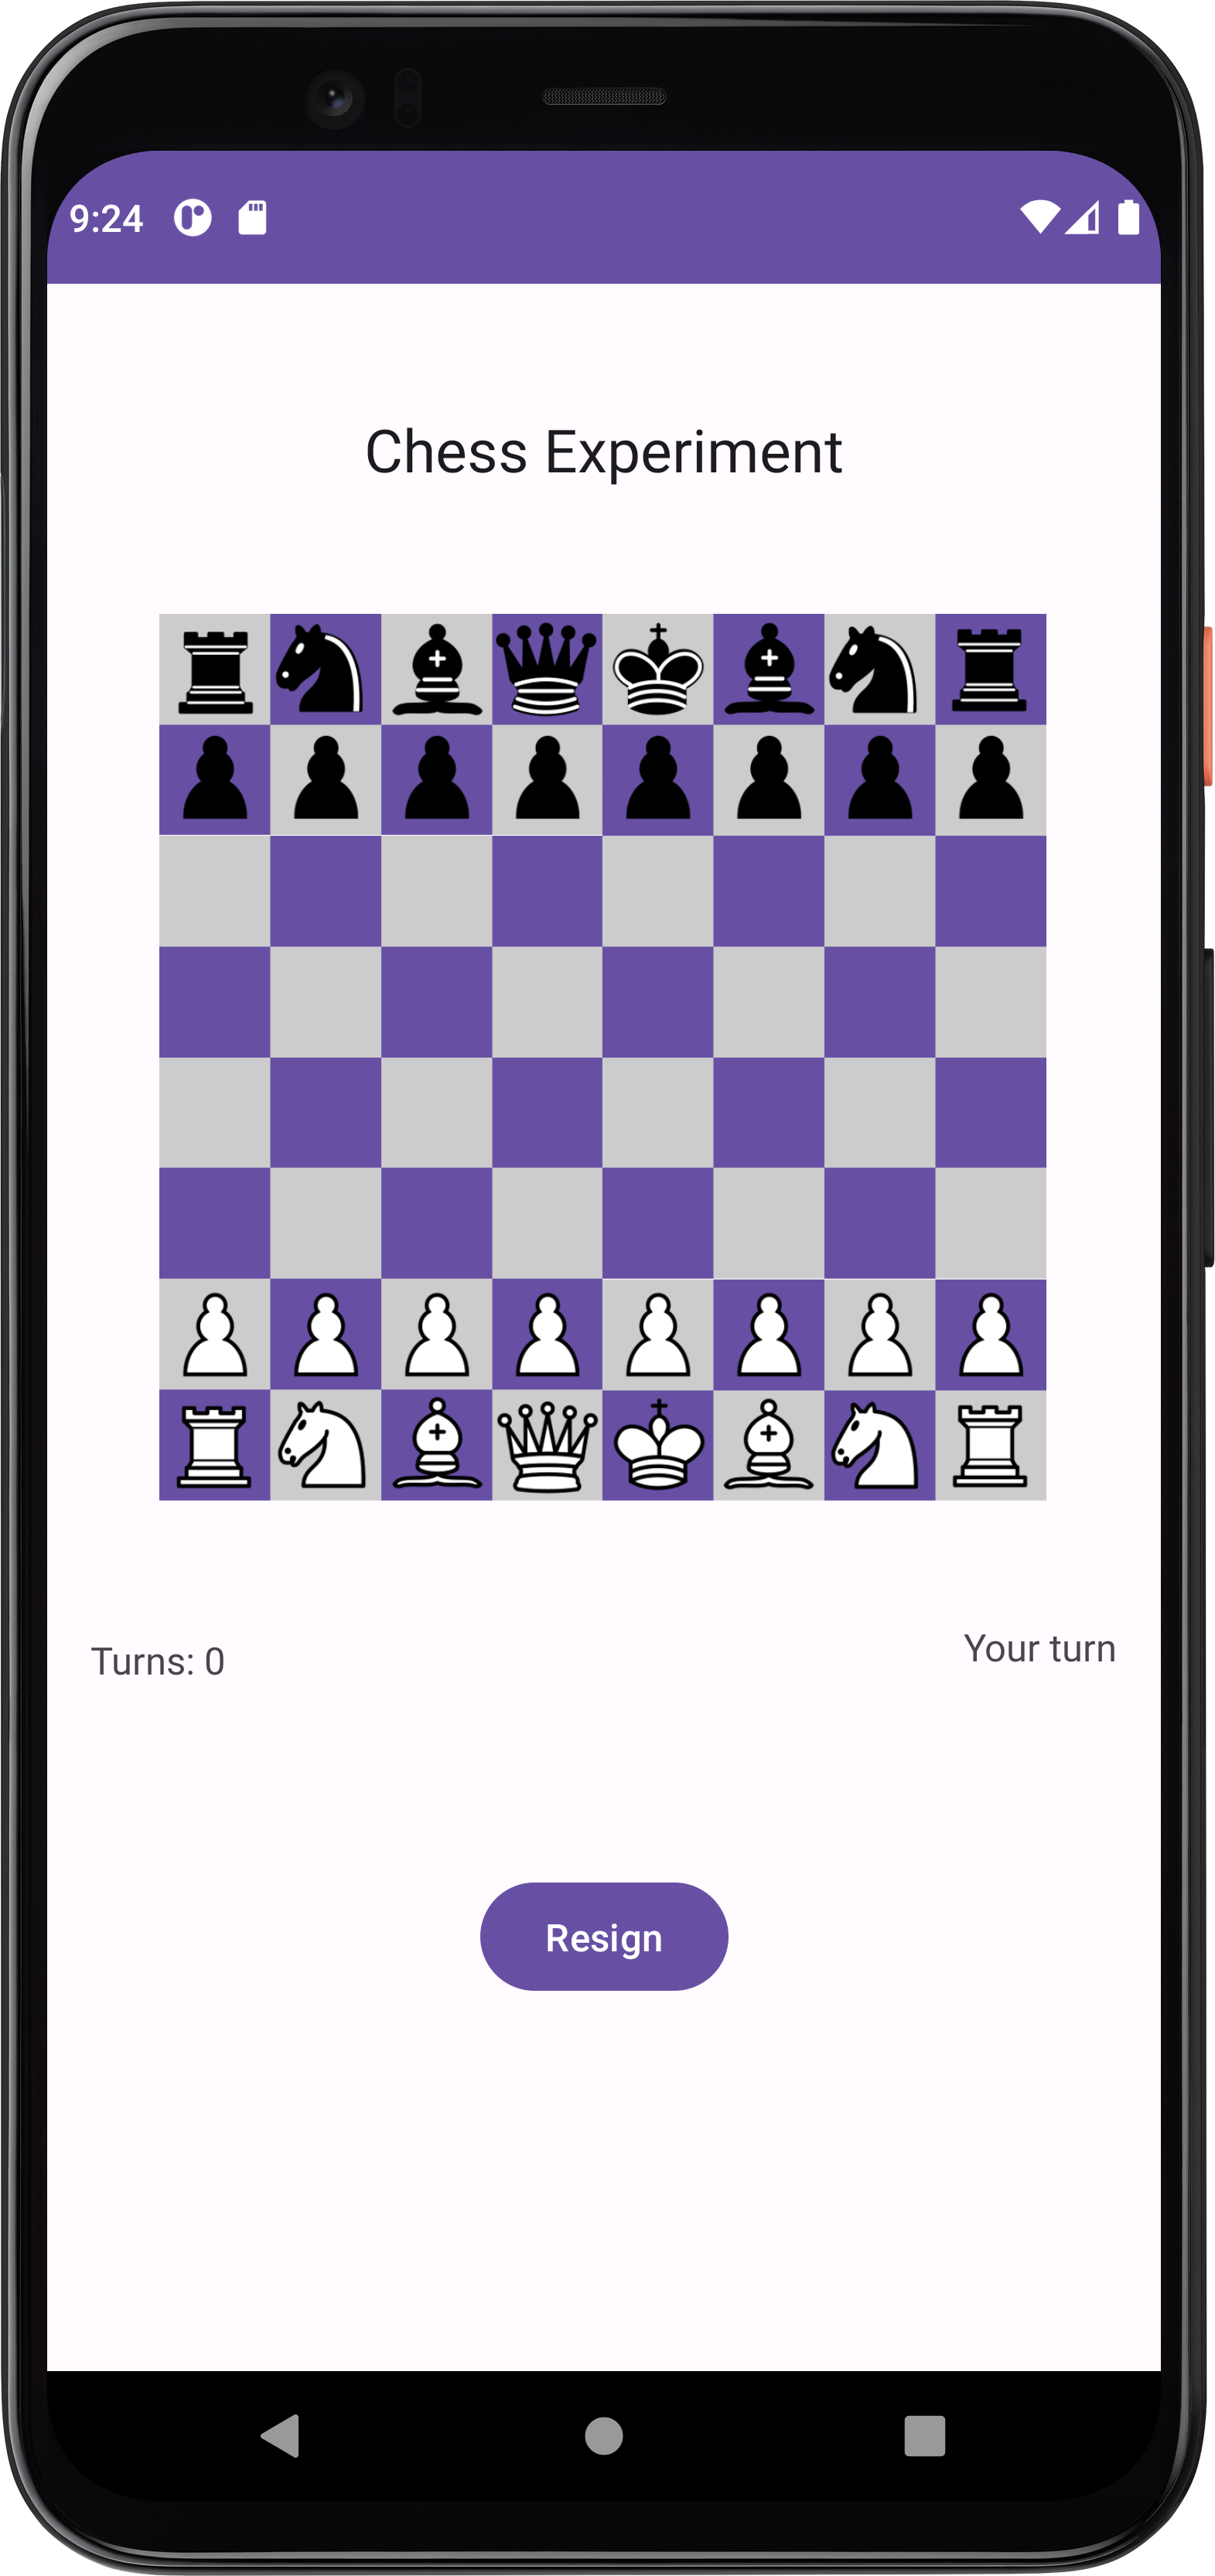
\includegraphics[width=0.3\textwidth, keepaspectratio]{content/07_evaluation_of_the_solution/Screenshot_Chess.png}
    \caption{Custom experiment logic}    
    \label{fig:chess}
\end{figure}

\begin{lstlisting}[language=java,label=t6,lineskip={0pt}, caption=Collect time needed to conduct experiment (b), basicstyle=\scriptsize, captionpos=b]
    currentParticipant = getCurrentParticipantUseCase.getCurrentParticipant();
    currentParticipantGroup = participantRepository.getParticipant(currentParticipant).getGroupAllocation();
    
    if(currentParticipantGroup == null){
    
        if(experimentRepository.getExperiment().getGroupAllocation() == "random"){
            Random random = new Random();
            int randomNumber = random.nextInt(2); // Generates either 0 or 1
    
            if(randomNumber == 0 ){
                setGroupAllocationPUseCase.setGroupAllocation("Group A", currentParticipant);
            } else {
                setGroupAllocationPUseCase.setGroupAllocation("Group B", currentParticipant);
            }
        };
    }
\end{lstlisting}


\begin{lstlisting}[language=java,label=t7b,lineskip={0pt}, caption=Collect time needed to conduct experiment (b), basicstyle=\scriptsize, captionpos=b]
    private class ClientThread extends Thread {
        @Override
        public void run() {
            try {
                Socket socket = new Socket(server_ip, server_port);
                PrintWriter out = new PrintWriter(socket.getOutputStream(), true);
                out.println(message);
                out.close();
                socket.close();
            } catch (IOException e) {
                e.printStackTrace();
            }
        }
    }
\end{lstlisting}

\begin{lstlisting}[language=java,label=t7a,lineskip={0pt}, caption=Collect time needed to conduct experiment (b), basicstyle=\scriptsize, captionpos=b]
private class ServerThread extends Thread {
        @Override
        public void run() {
            try {
                ServerSocket serverSocket = new ServerSocket(client_port);
                Socket clientSocket = serverSocket.accept();

                BufferedReader in = new BufferedReader(new InputStreamReader(clientSocket.getInputStream()));
                String message = in.readLine();
                in.close();
                clientSocket.close();
                serverSocket.close();

                handleMessage(message);

            } catch (IOException e) {
                e.printStackTrace();
            }
        }
    }
\end{lstlisting}

\begin{lstlisting}[language=java,label=t7c,lineskip={0pt}, caption=Collect time needed to conduct experiment (b), basicstyle=\scriptsize, captionpos=b]
    new ClientThread().start();
    new ServerThread().start();
\end{lstlisting}

\begin{lstlisting}[language=java,label=t8,lineskip={0pt}, caption=Collect time needed to conduct experiment (b), basicstyle=\scriptsize, captionpos=b]
    File file = new File(Environment.getExternalStorageDirectory() + "/participant" + GetCurrentParticipantUseCase.getInstance().getCurrentParticipant() + "TimeData.csv");
    try {
        // create FileWriter object with file as parameter
        FileWriter outputfile = new FileWriter(file);

        // create CSVWriter object filewriter object as parameter
        CSVWriter writer = new CSVWriter(outputfile);

        // adding header to csv
        String[] header = { "id", "time in milliseconds"};
        writer.writeNext(header);

        //Getting participant information
        ArrayList<ParticipantEntity> participantEntities = GetParticipantDataUseCase.getInstance().getParticipantData();

        //Writing current participant time into file
        //String[] data = {String.valueOf(GetCurrentParticipantUseCase.getInstance().getCurrentParticipant()), String.valueOf(timeDifference)};

        Iterator iter = participantEntities.iterator();
        while (iter.hasNext()) {
            String[] data = {String.valueOf(((ParticipantEntity)iter.next()).getId()), String.valueOf(((ParticipantEntity)iter.next()).getExperimentTime())};
            writer.writeNext(data);
        }
        //closing writer connection
        writer.close();
    }
    catch (IOException e) {
        // TODO Auto-generated catch block
        e.printStackTrace();
        System.out.println("Error");
    }
\end{lstlisting}

\begin{figure}[htbp]
    \centering
    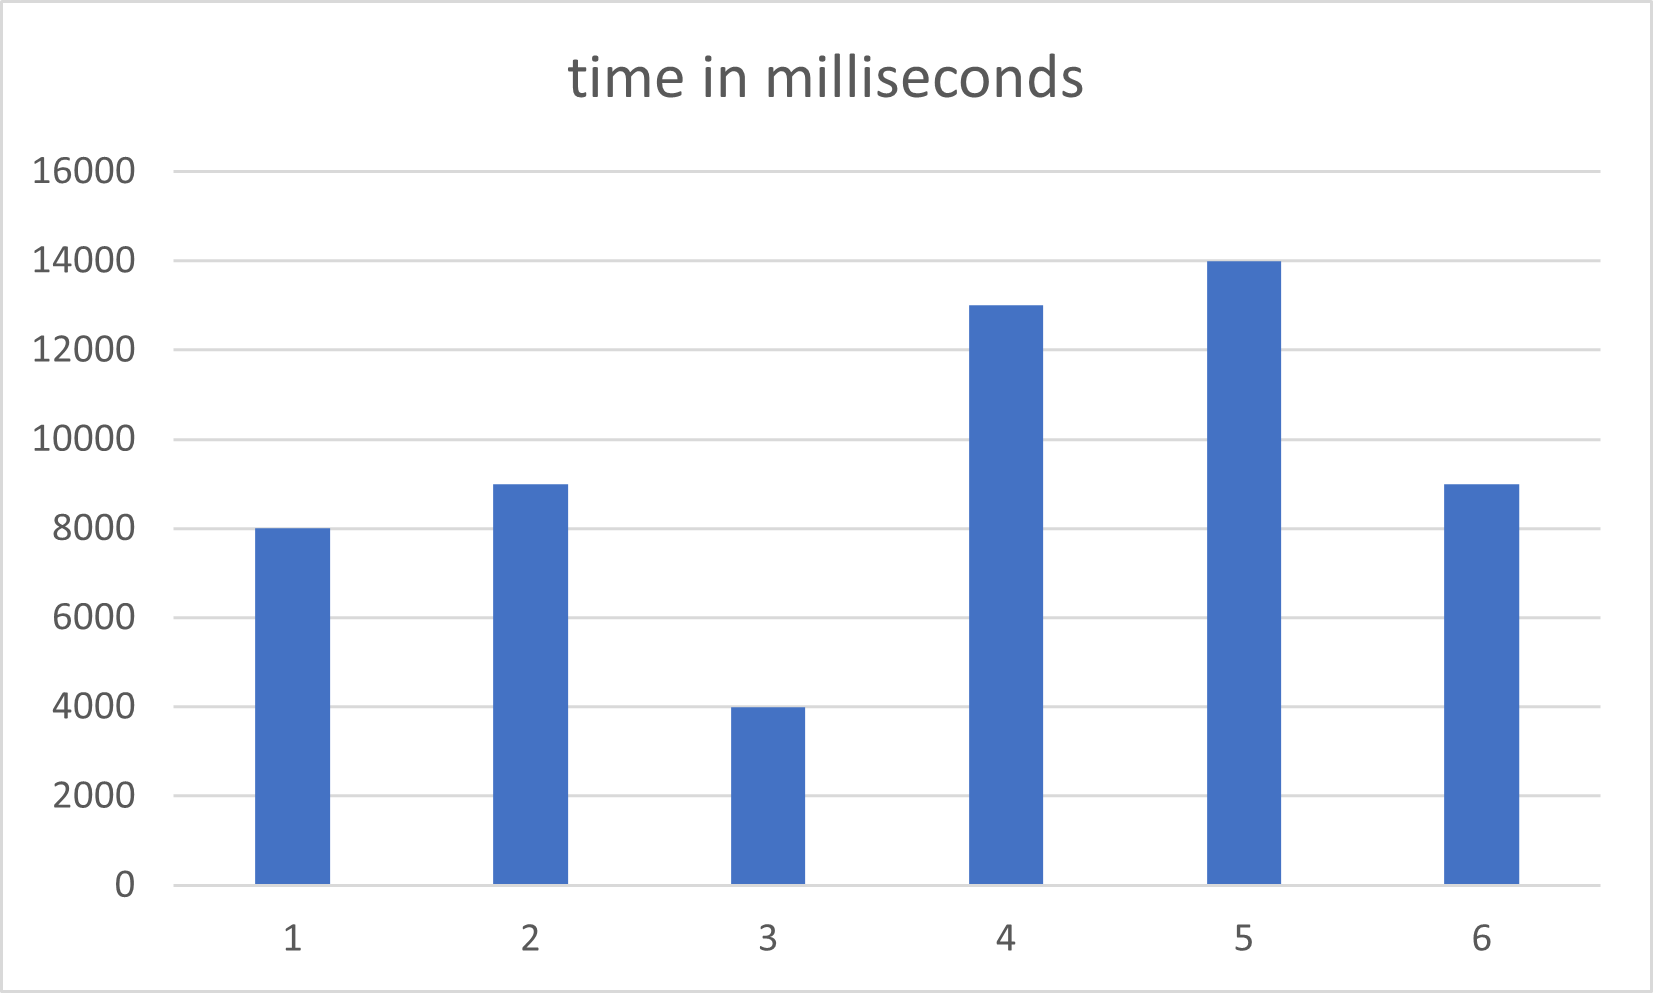
\includegraphics[width=0.99\textwidth, keepaspectratio]{content/07_evaluation_of_the_solution/ExcelPicture.png}
    \caption{Data loaded into excel}    
    \label{fig:Excel}
\end{figure}

\begin{figure}[htbp]
    \centering
    \begin{subfigure}[b]{0.25\textwidth}
        \centering
        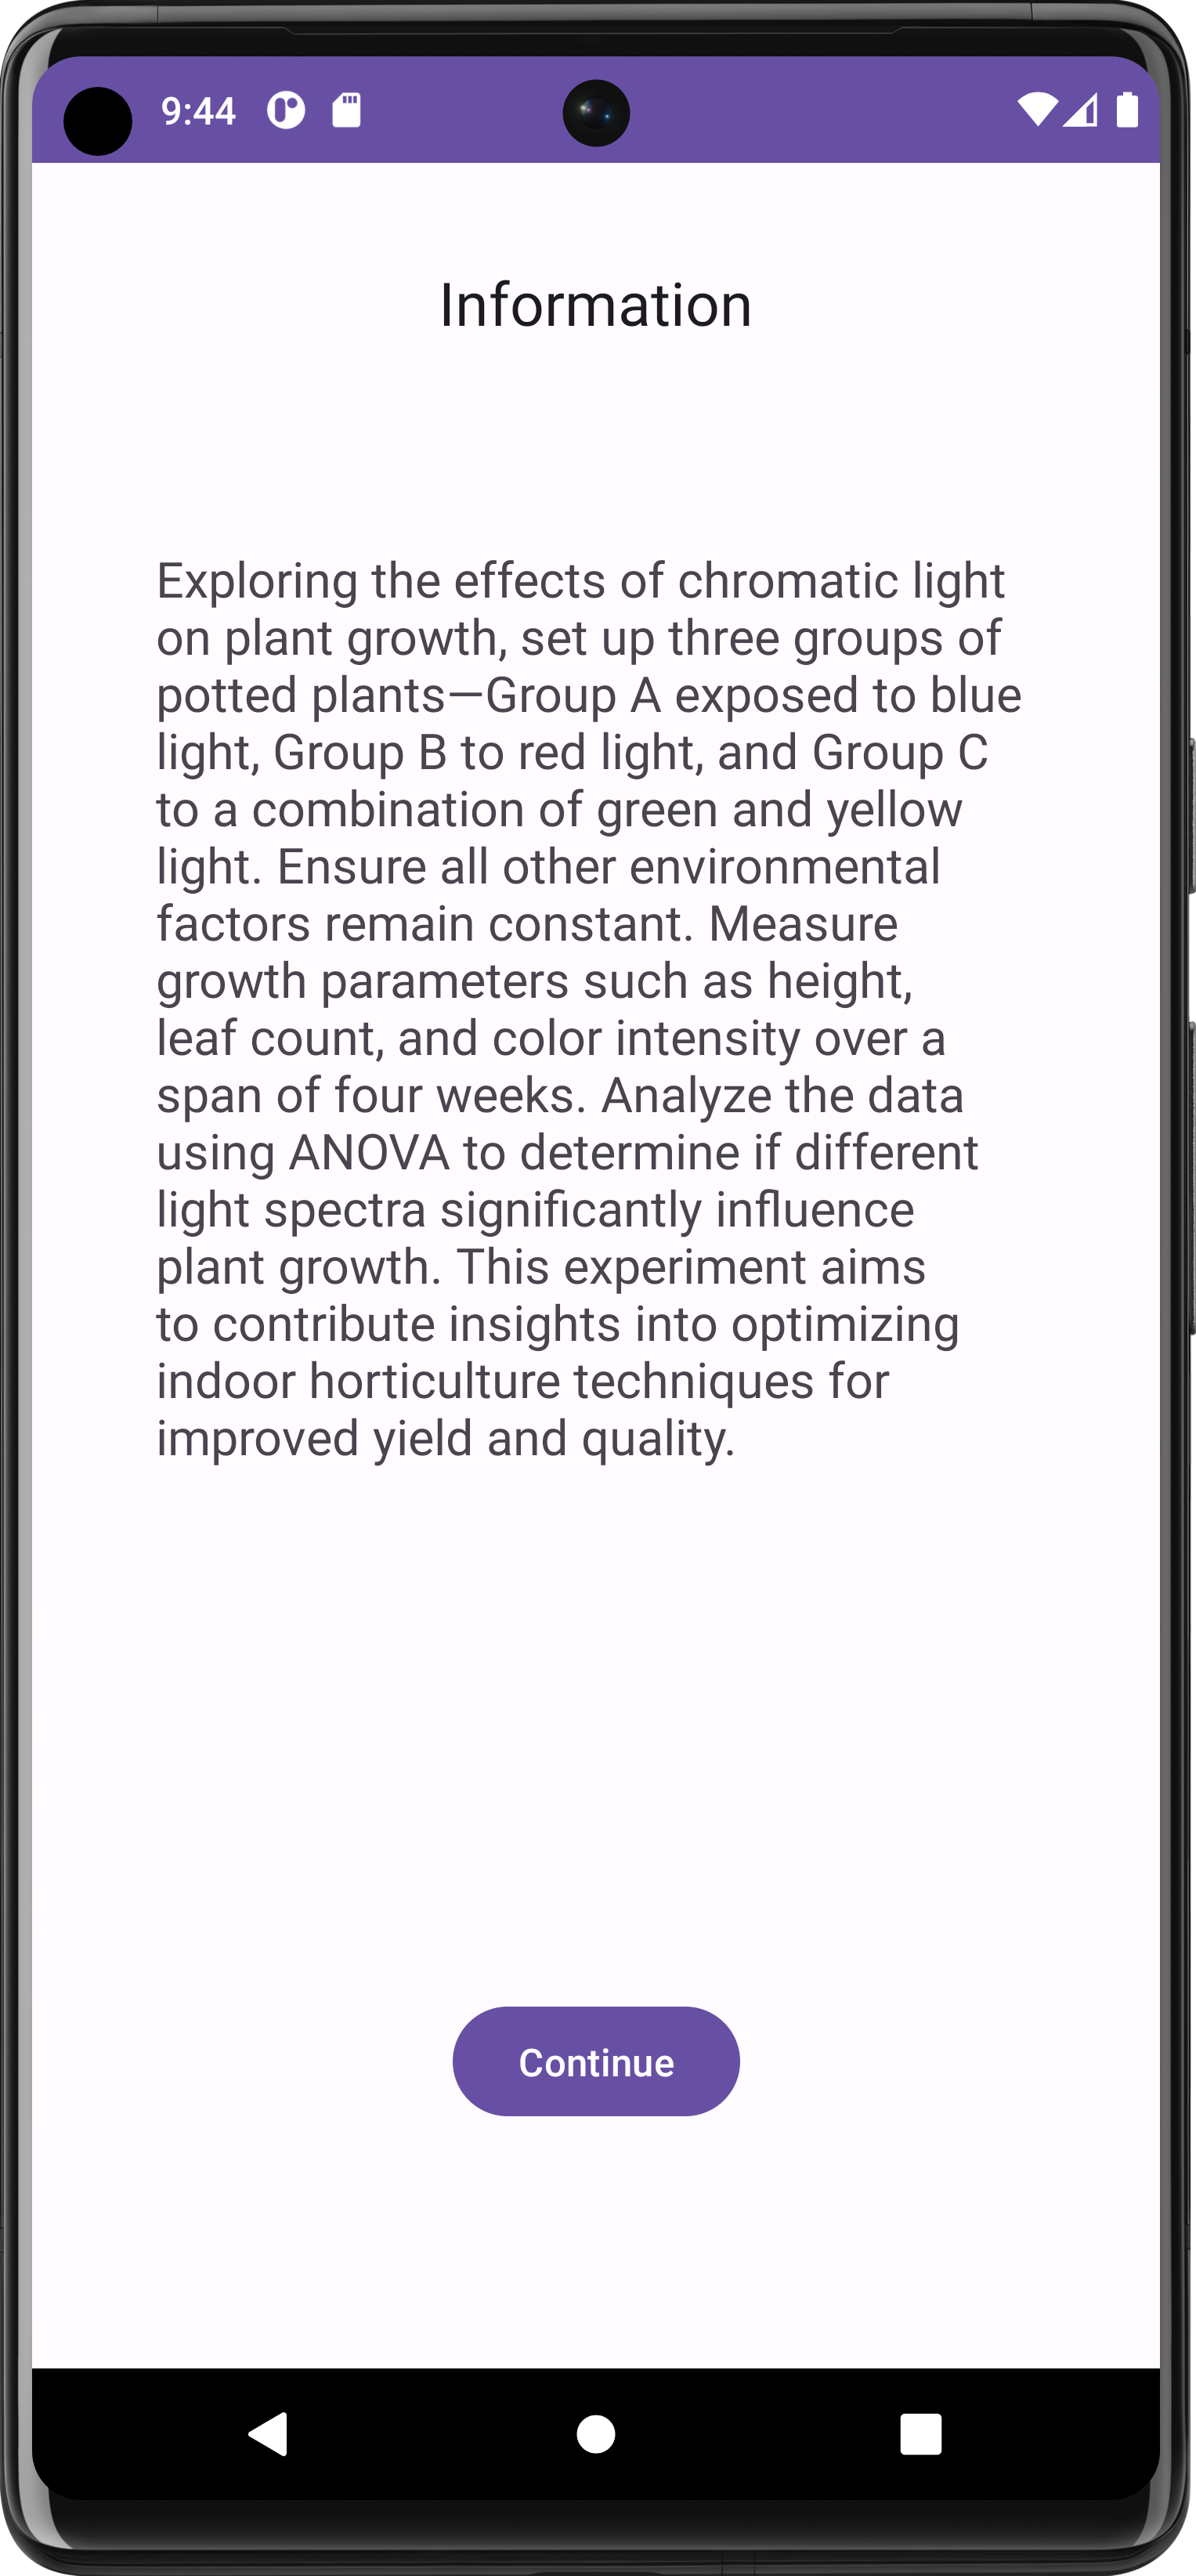
\includegraphics[width=\textwidth]{content/07_evaluation_of_the_solution/Screenshot_T10a.png}
        \caption{Info screen step | Pixel 6 Pro}
        \label{subfig:InfoScreenPixel}
    \end{subfigure}
        %\hfill
        \hspace{1cm}
    \begin{subfigure}[b]{0.25\textwidth}
        \centering
        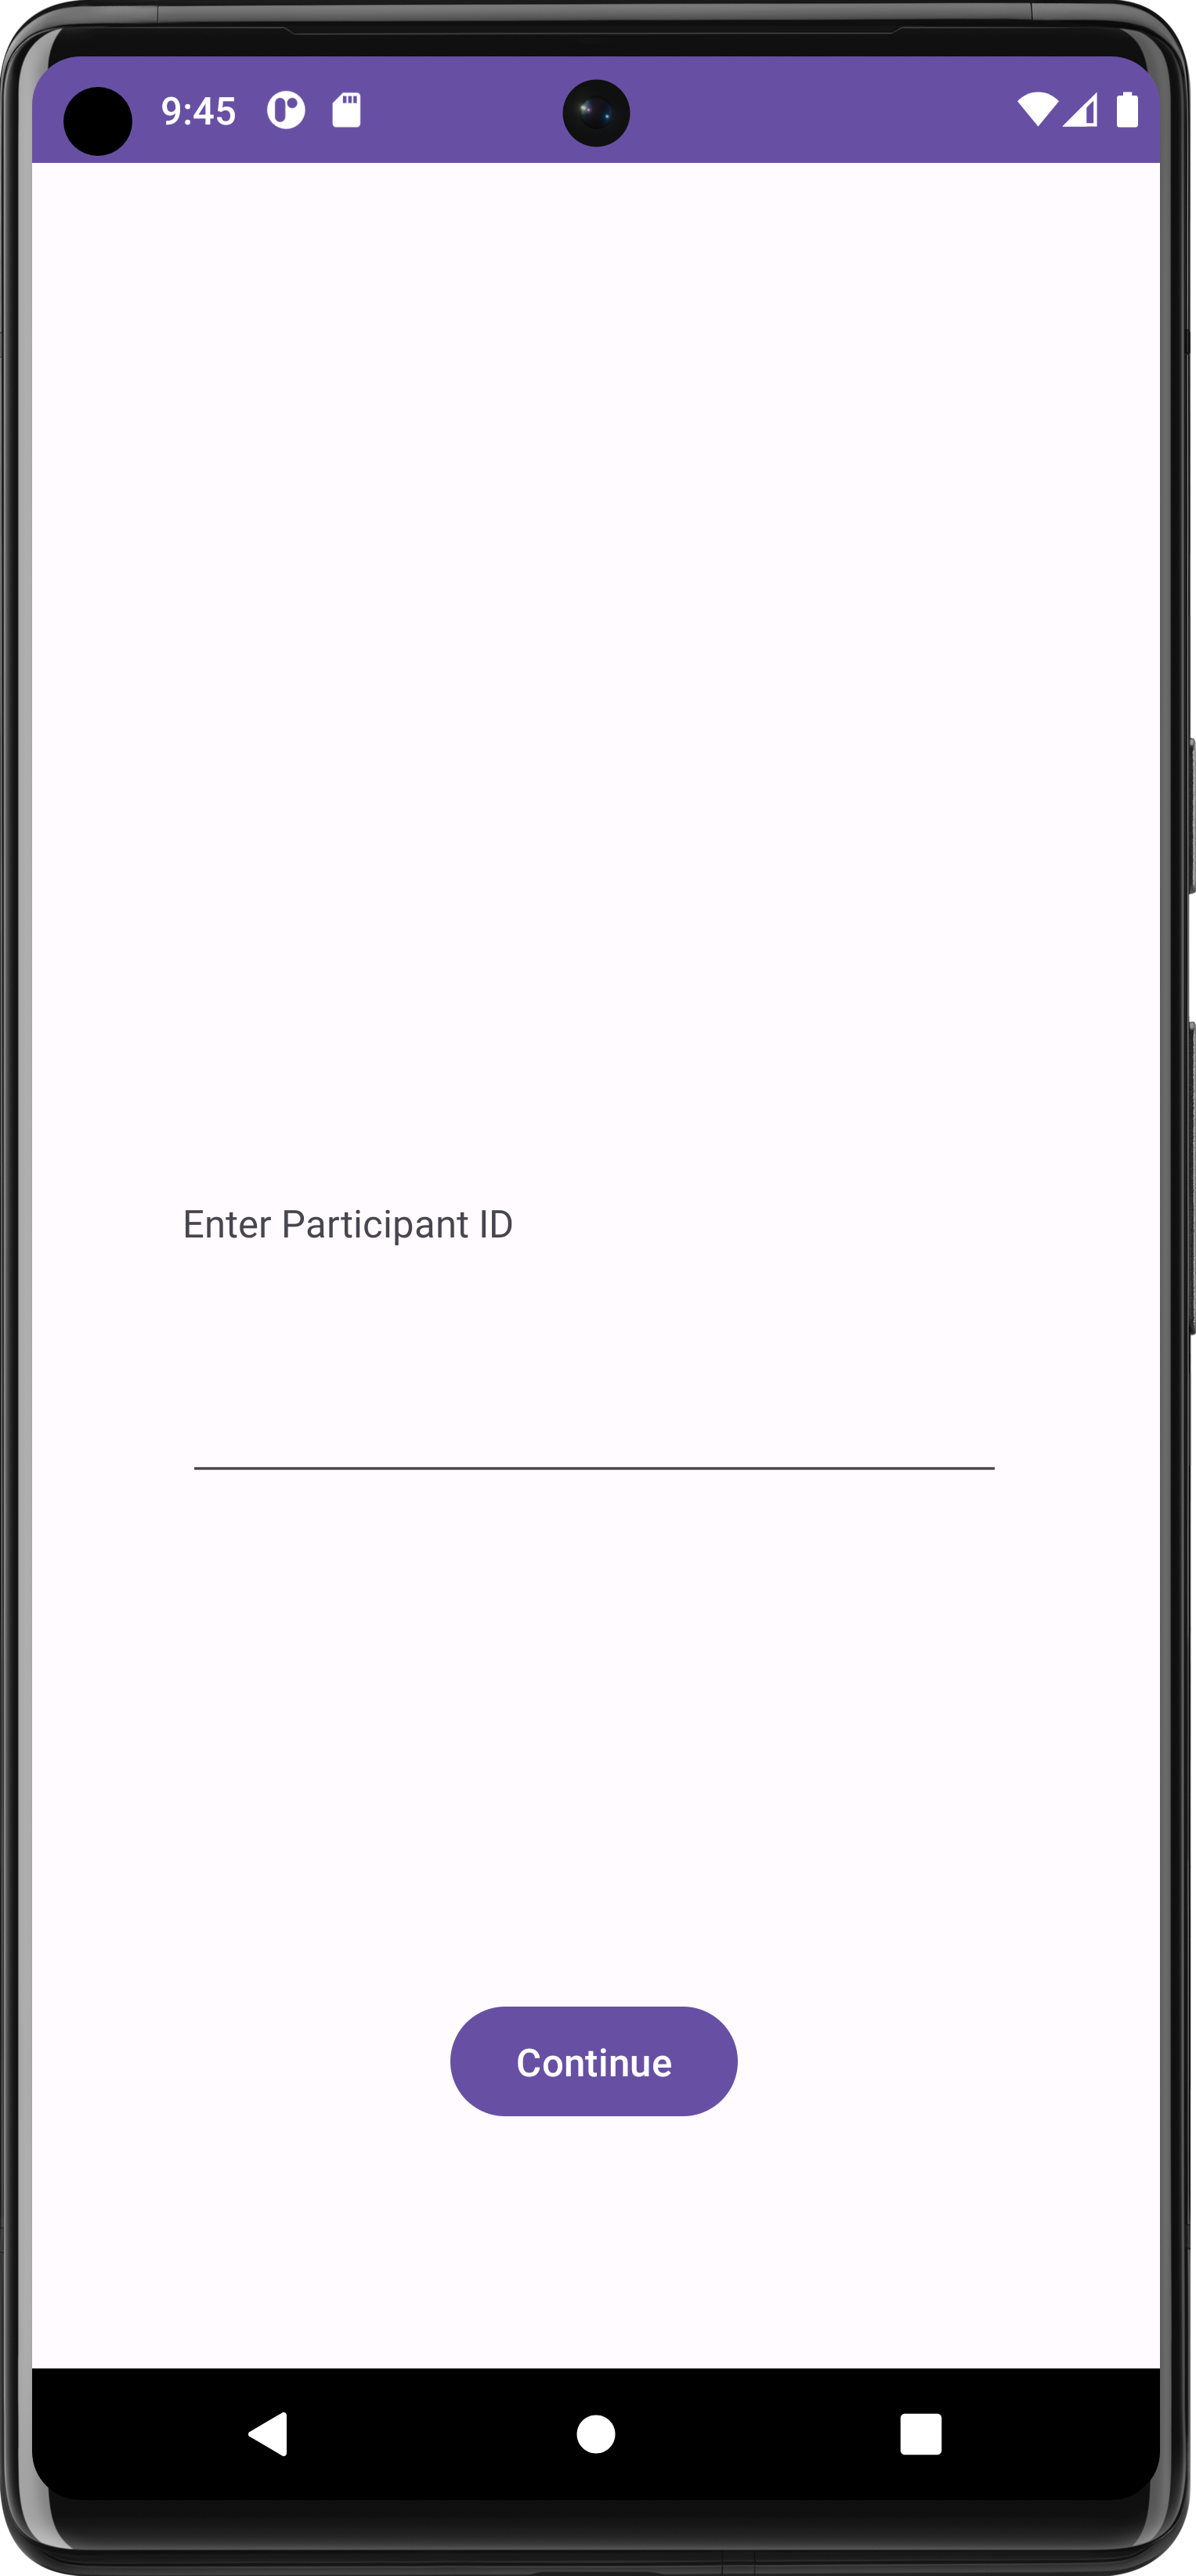
\includegraphics[width=\textwidth]{content/07_evaluation_of_the_solution/Screenshot_T10b.png}
        \caption{ Questionair step | Pixel 6 Pro}
        \label{subfig:QuestionairPixel}
    \end{subfigure}
        %\hfill
        \hspace{1cm}
    \begin{subfigure}[b]{0.25\textwidth}
        \centering
        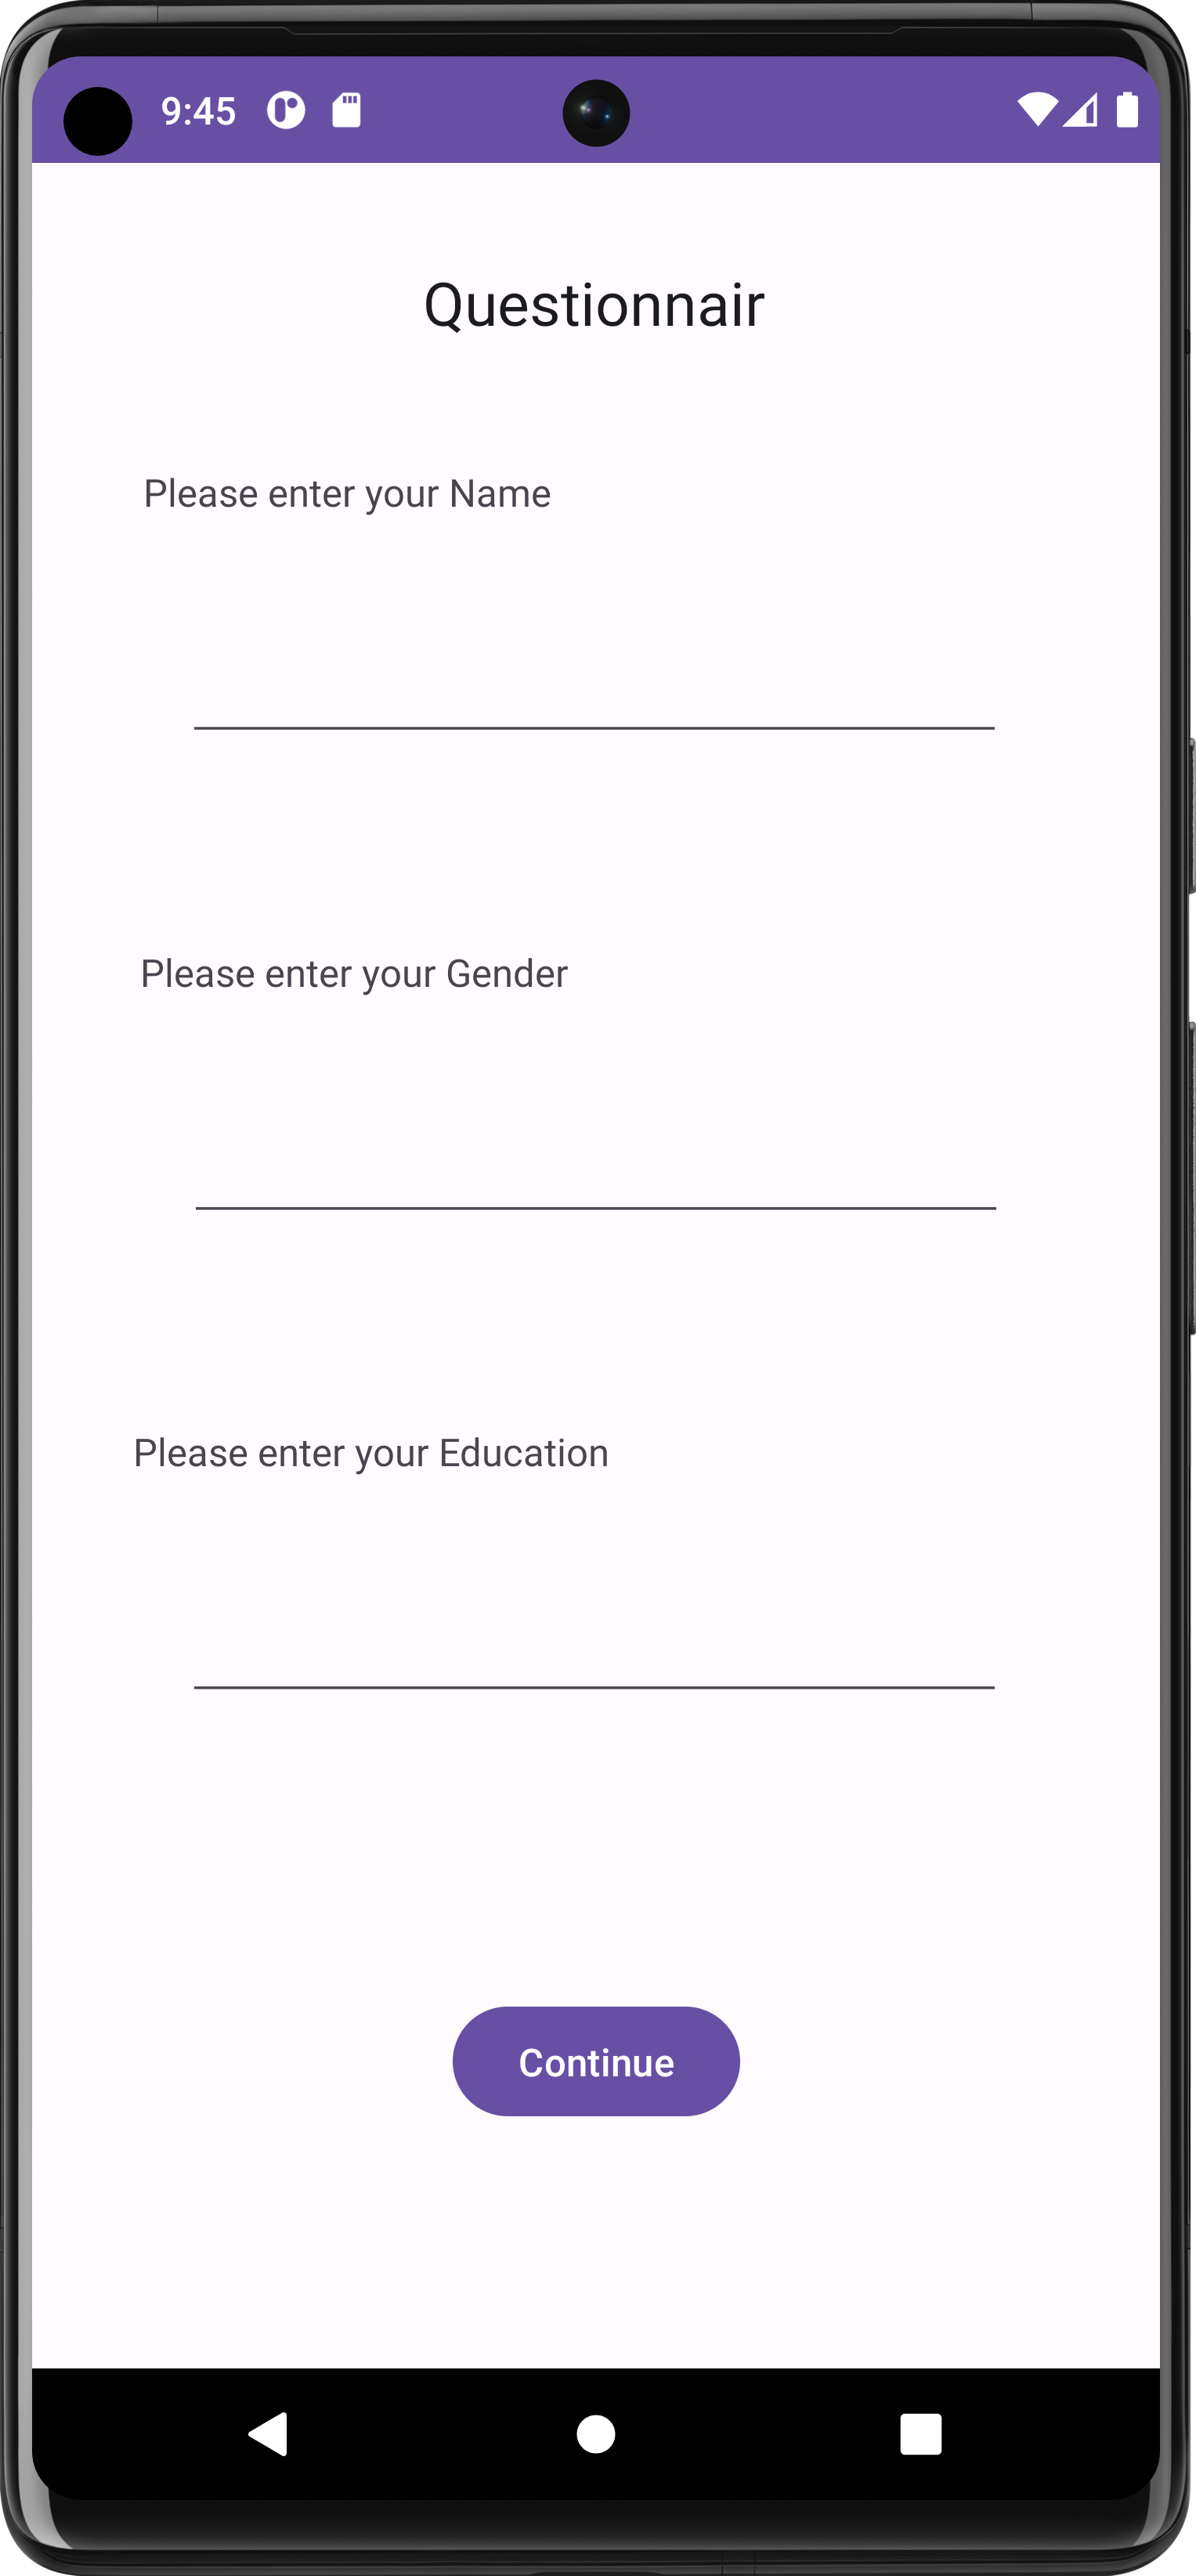
\includegraphics[width=\textwidth]{content/07_evaluation_of_the_solution/Screenshot_T10c.png}
        \caption{Choose test subject step | Pixel 6 Pro}
        \label{subfig:chooseTestSubjectPixel}
    \end{subfigure}
       \caption{Artefact run on a Pixel 6 Pro}
       \label{fig:uiScreensPixel6}
\end{figure}

\begin{figure}[htbp]
    \centering
    \begin{subfigure}[b]{0.25\textwidth}
        \centering
        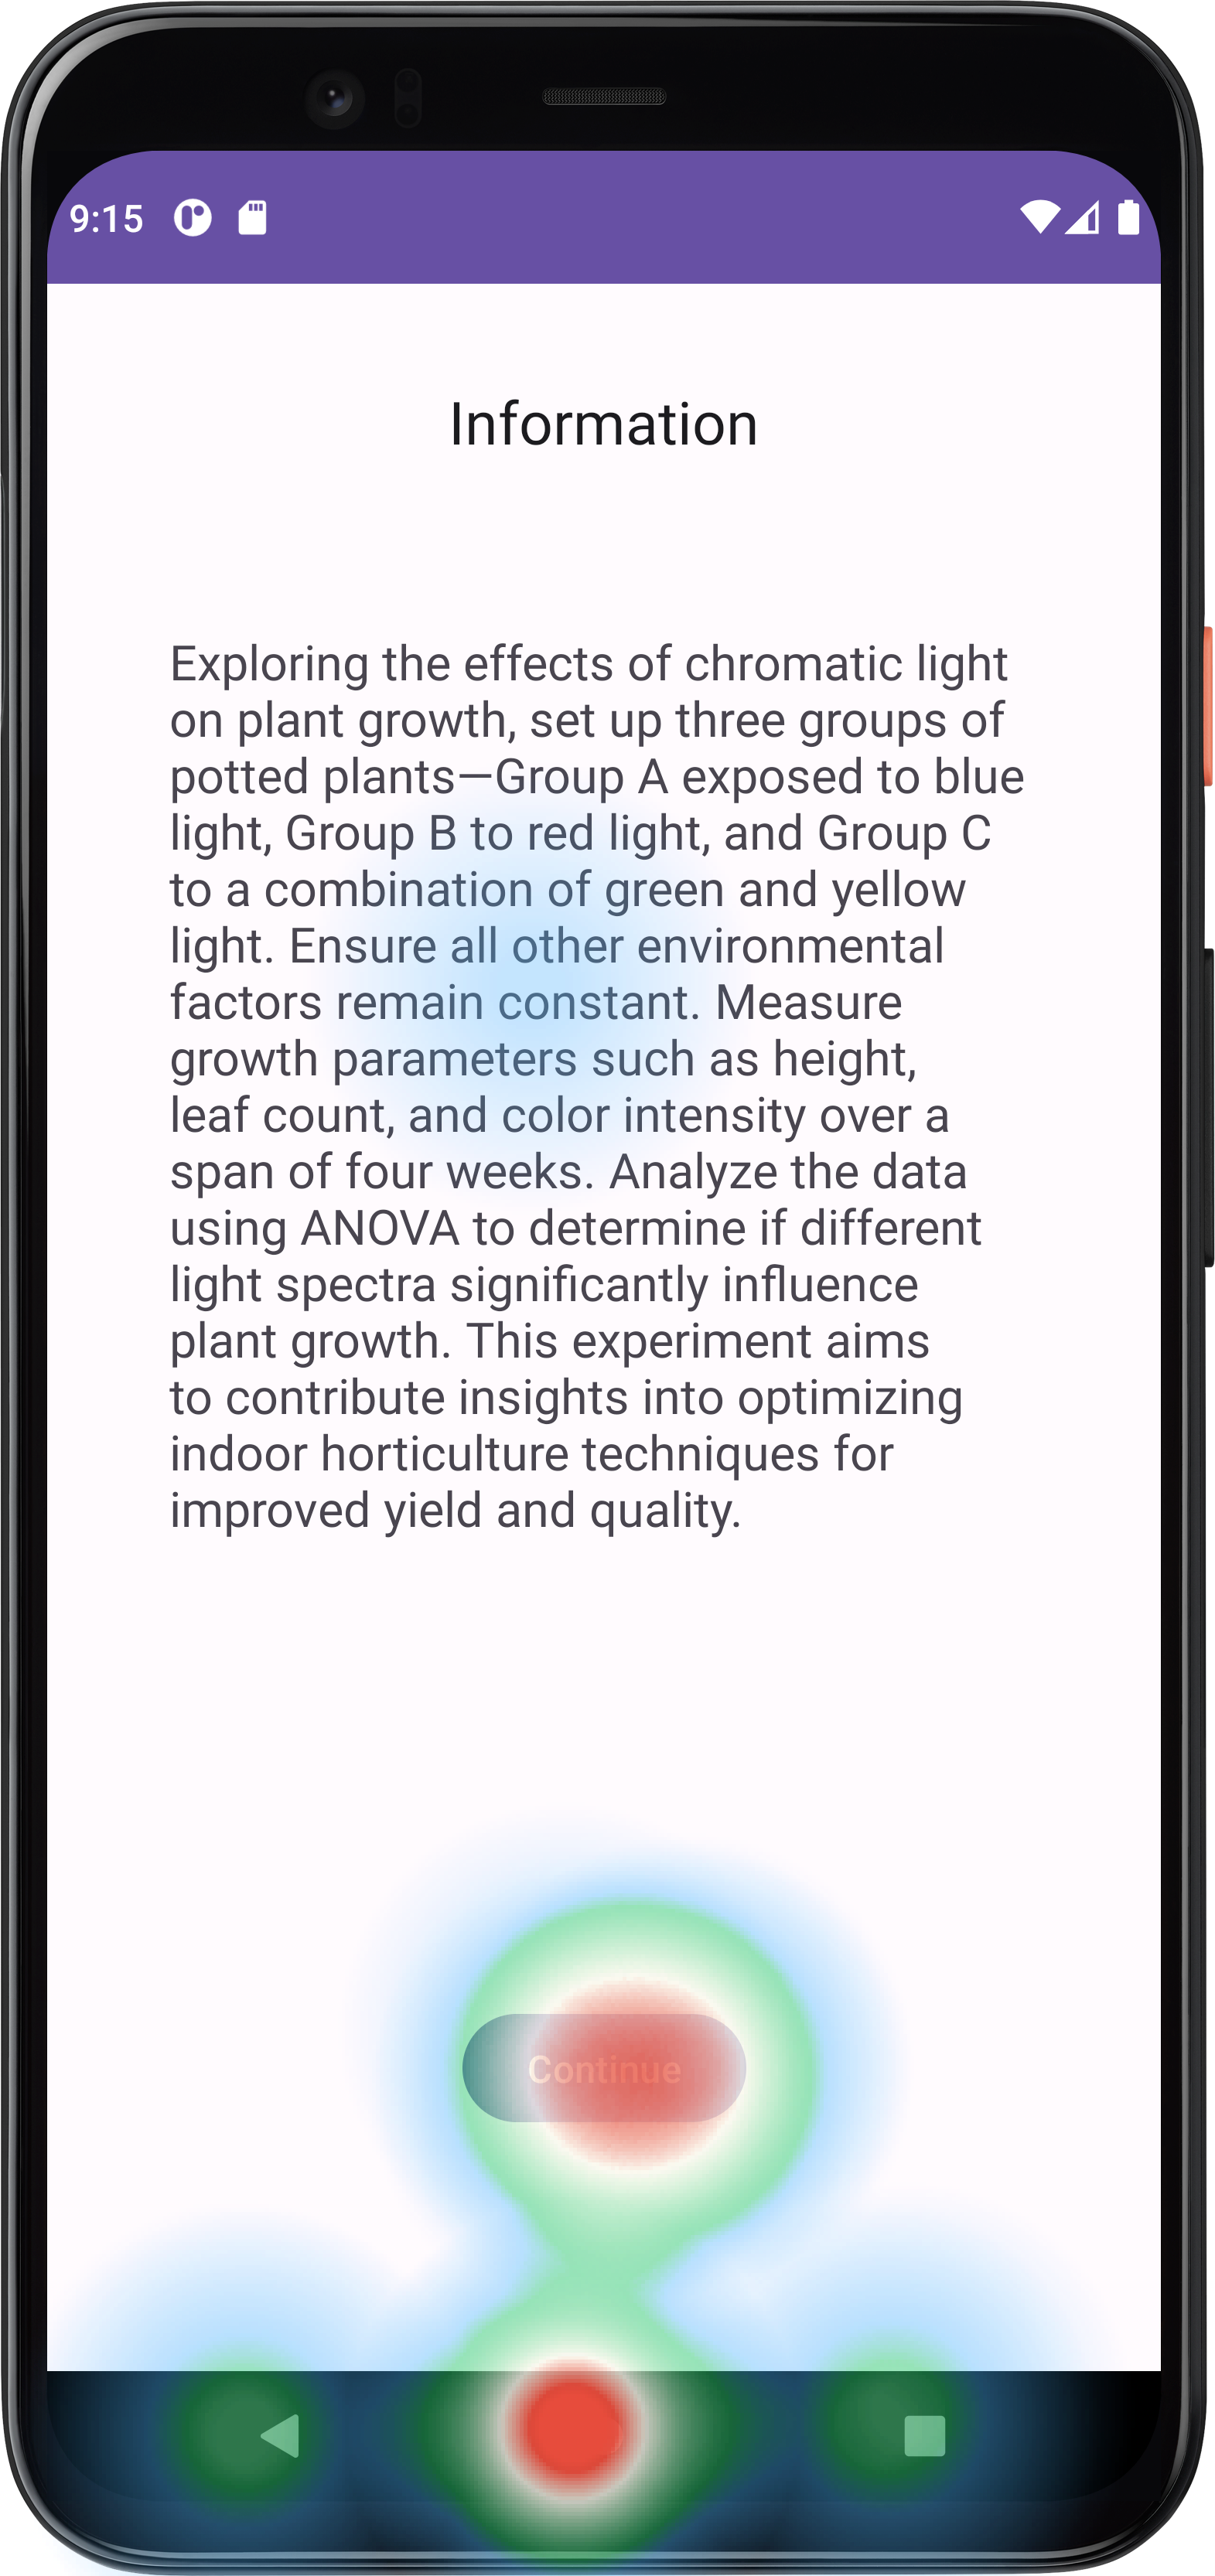
\includegraphics[width=\textwidth]{content/07_evaluation_of_the_solution/HeatMap_InfoScreen.png}
        \caption{Info Screen}
        \label{subfig:heatmapA}
    \end{subfigure}
        %\hfill
        \hspace{1cm}
    \begin{subfigure}[b]{0.25\textwidth}
        \centering
        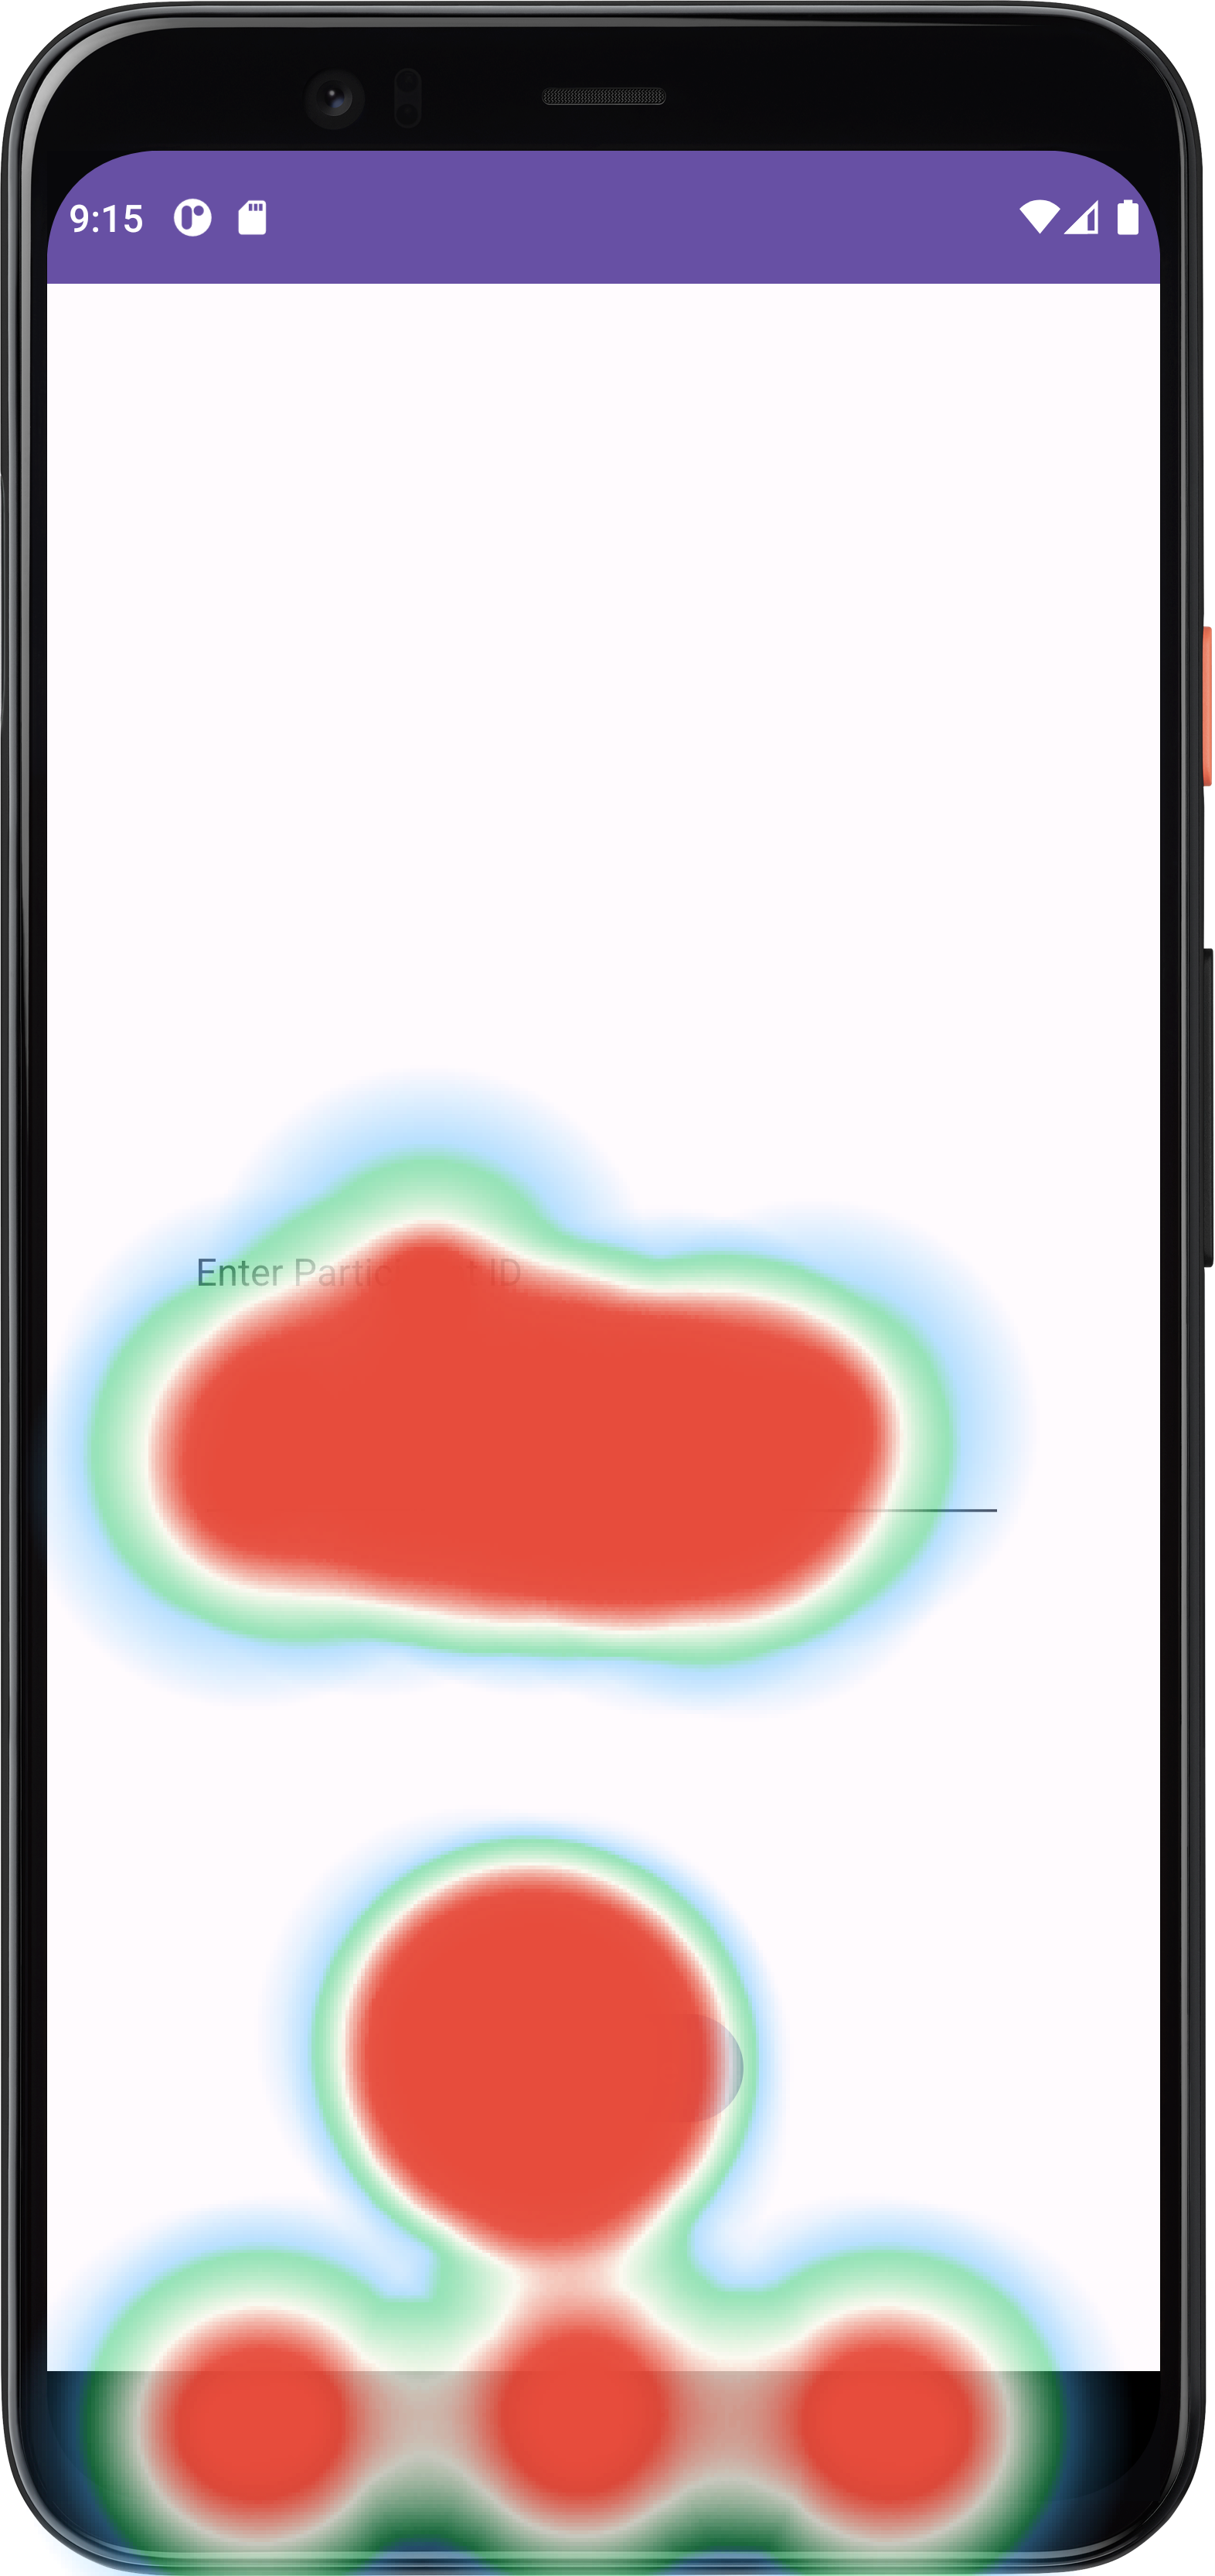
\includegraphics[width=\textwidth]{content/07_evaluation_of_the_solution/HeatMap_ParticipantSelectionScreen.png}
        \caption{Participant Selection}
        \label{subfig:heatmapB}
    \end{subfigure}
        %\hfill
        \hspace{1cm}
    \begin{subfigure}[b]{0.25\textwidth}
        \centering
        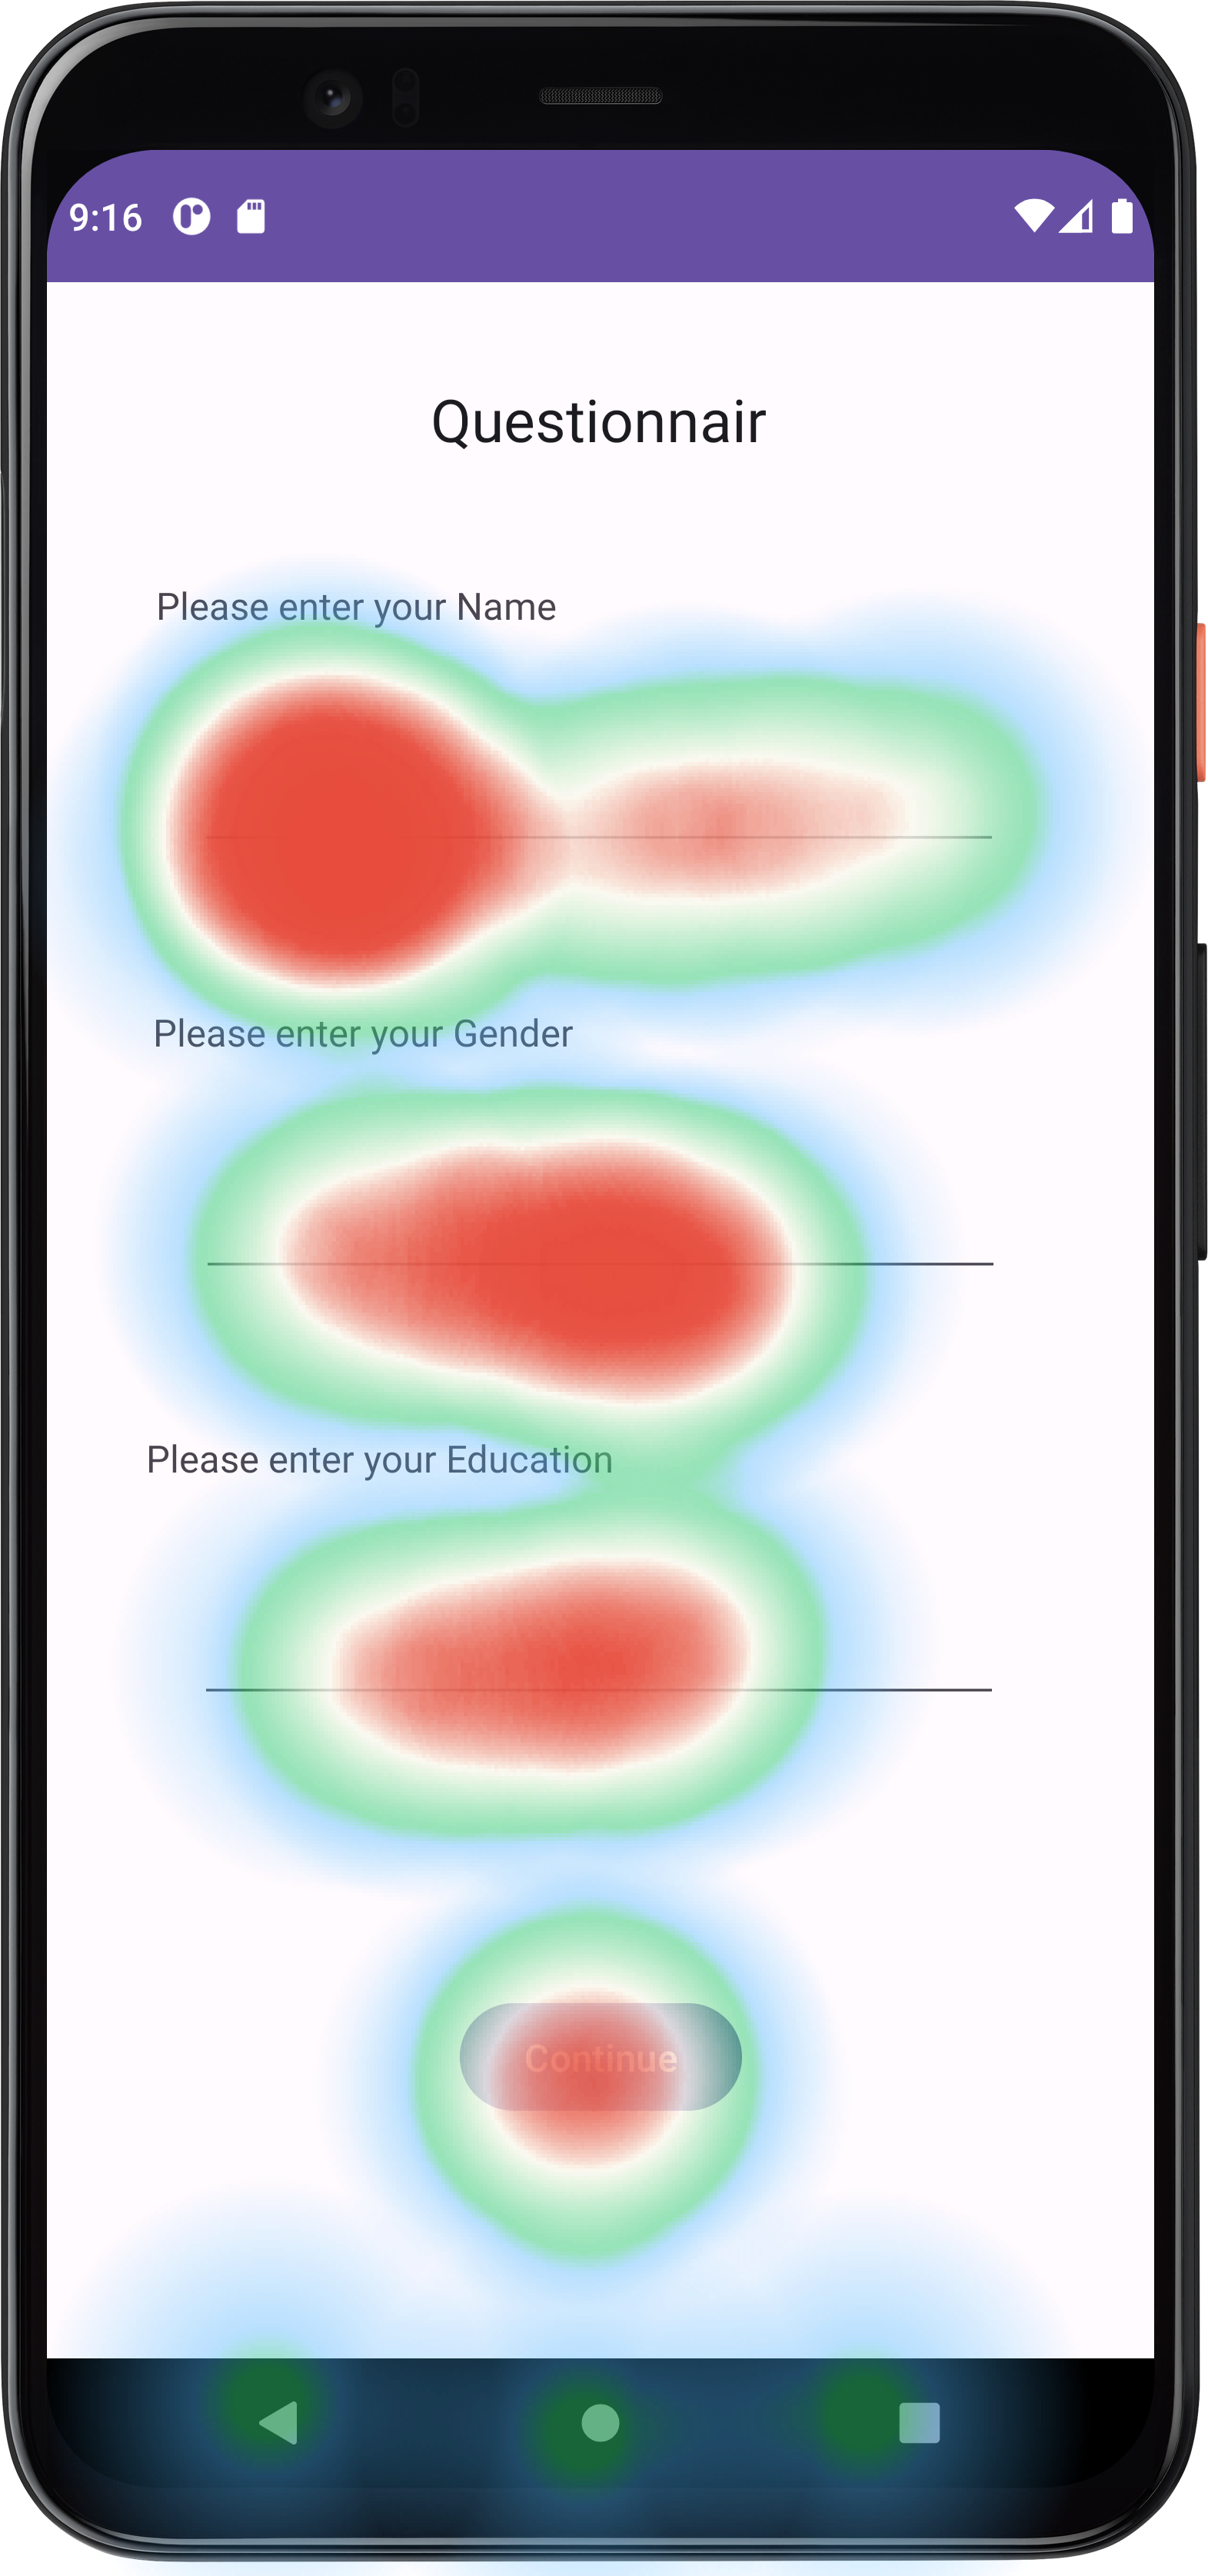
\includegraphics[width=\textwidth]{content/07_evaluation_of_the_solution/HeatMap_QuestionnairScreen.png}
        \caption{Questionnair Step}
        \label{subfig:heatmapC}
    \end{subfigure}
       \caption{Heatmaps}
       \label{fig:heatmaps}
\end{figure}